\section{Overview}
The architecture of the S\&C system is presented in this section.
\begin{figure}[H]
    \centering
    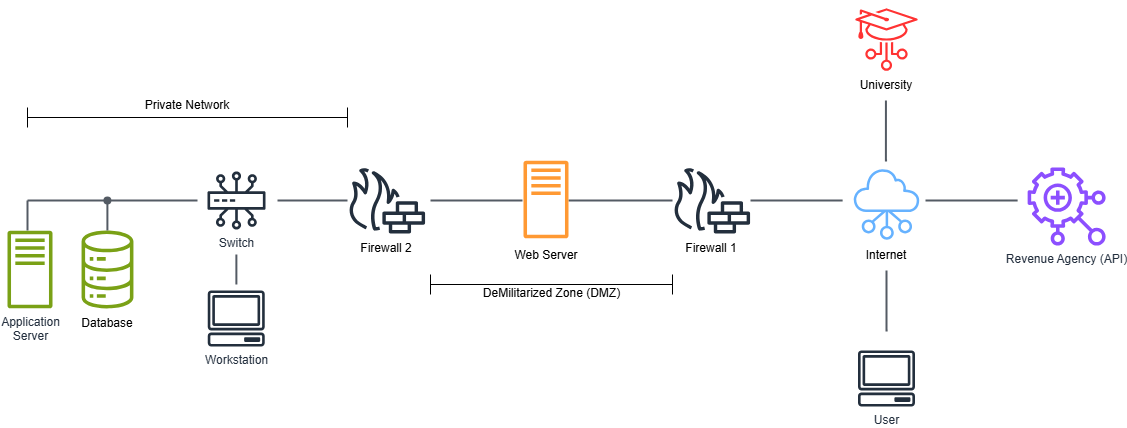
\includegraphics[width=15cm]{images/architectural design/overview.png}
    \caption{Overview of the S\&C system}
\end{figure}
This diagram illustrates the platform's entire architecture, highlighting how the components are interconnected and how security is ensured. 
The \textbf{Private Network} is the backbone of the platform. It hosts the \textbf{Application Server}, which runs the system's logic, and the \textbf{Database} where all the data is stored. These components are connected via a switch to a Workstation used for internal administration, such as company registrations.\newline
The \textbf{Demilitarized Zone} (DMZ) contains the Web Server, which handles user requests. 
The DMZ is placed between the two firewalls. This is standard practice to ensure that external users can only access the components within the DMZ (in this case, the Web Server) while maintaining the security of components inside the Private Network.\newline
On the \textbf{Internet}-facing side, the platform interacts with users and integrates with external services, such as the university SSO systems and the Revenue Agency APIs.
\pagebreak
\section{Component view}
\begin{figure}[H]
    \centering
    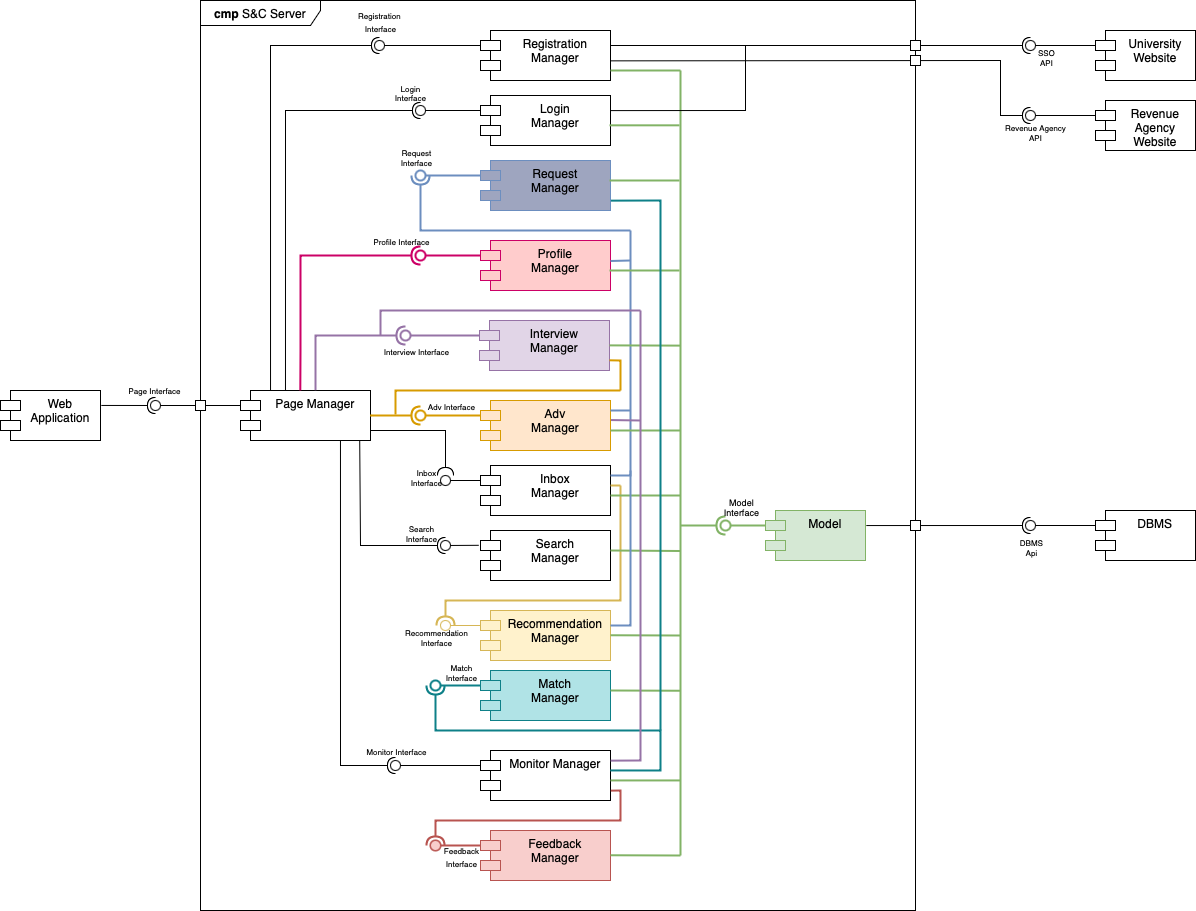
\includegraphics[width=15cm]{images/architectural design/DD-ArchitecturalManager.png}
    \caption{Component view: Low Level Diagram}
    \label{figure:LowLevelDiagram}
\end{figure}
The figure \ref{figure:LowLevelDiagram} represent the S\&C architecture the Server's components:
\begin{itemize}
    \item \textbf{Page Manager:} This component directs the User's requests through the Page Interface to the correct component. It acts like a switch for whole the server.
    
    \item \textbf{Registration Manager:} This component handles new User registration, receiving the request from the Page Manager, and communicating with the university SSO API, if the user is a Student or with the Revenue Agency API, if the user is a Company. This component communicates also with the Users DBMS saving information about the new User.

    \item \textbf{Login Manager:} This component handles the login of an existing User, it communicates with the Users DBMS in order to check the validity of the credentials used by the User.

    \item \textbf{Request Manager:} This component is responsible for managing the Request of a Company to contact a Student and vice versa. If a Request is accepted the creation of a Match will be triggered.

    \item \textbf{Profile Manager:} This component loads the Profile Page of both Students and Companies by communicating with the Users DBMS. This component, also, communicates with Request Manager in order to create a Request in case a visitor of the profile wants to contact the owner.

    \item \textbf{Interview Manager:} This component handles the request from the Adv Manager regarding the creation of a new Interview Form by the Users (C) and manages the interview requests.

    \item \textbf{Adv Manager:} This component handles the requests regarding the Adv Page: it loads the page by communicating with the DBMS, uses Request's interface to allow User (S) to send Requests to the Company proposing the Adv, and allow User (C) to create the Interview form thanks to Interview Manager's interface.

    \item \textbf{Inbox Manager:} This component handles the requests by the Page Manager regarding the Inbox Page that is loaded communicating with the DBMS. Also, it communicates with Request and Recommendation Manager to allow User to answer an internship request and contact the Users suggested in the Recommendation.

    \item \textbf{Search Manager:} This component handles the Page Manager's request about Search Page, and collects the results of the research made by the User by communicating with the DBMS.

    \item \textbf{Recommendation Manager:} This component handles the creation of recommendations using the data in the DBMS, uses the interface of Request Manager to let Users contact the suggestions made in the recommendation, and supplies to the Inbox Manager an interface to load the recommendation page.

    \item \textbf{Match Manager:} This component handles the request from the Monitor Manager regarding the information about a Match state by communicating with the DBMS.

    \item \textbf{Monitor Manager:} This component handles the requests by the Page Manager regarding the Monitor Page that is loaded communicating with the DBMS, Match Manager and Interview Manager. Also, it communicates with Feedback Manager in order to allow User to leave a feedback in certain states of the Match.

    \item \textbf{Feedback Manager:} This component handles the request from the Monitor Manager regarding the creation of a new Feedback from the Users.

    \item \textbf{Model:} This component handles the communication with the DBMS to fulfill all the requests of the other components about saving, deleting, getting or modifying data.
    
\end{itemize}
\pagebreak
\section{Deployment view}
Here follows the \textbf{Deployment Diagram} of the S\&C system.
\begin{figure}[H]
    \centering
    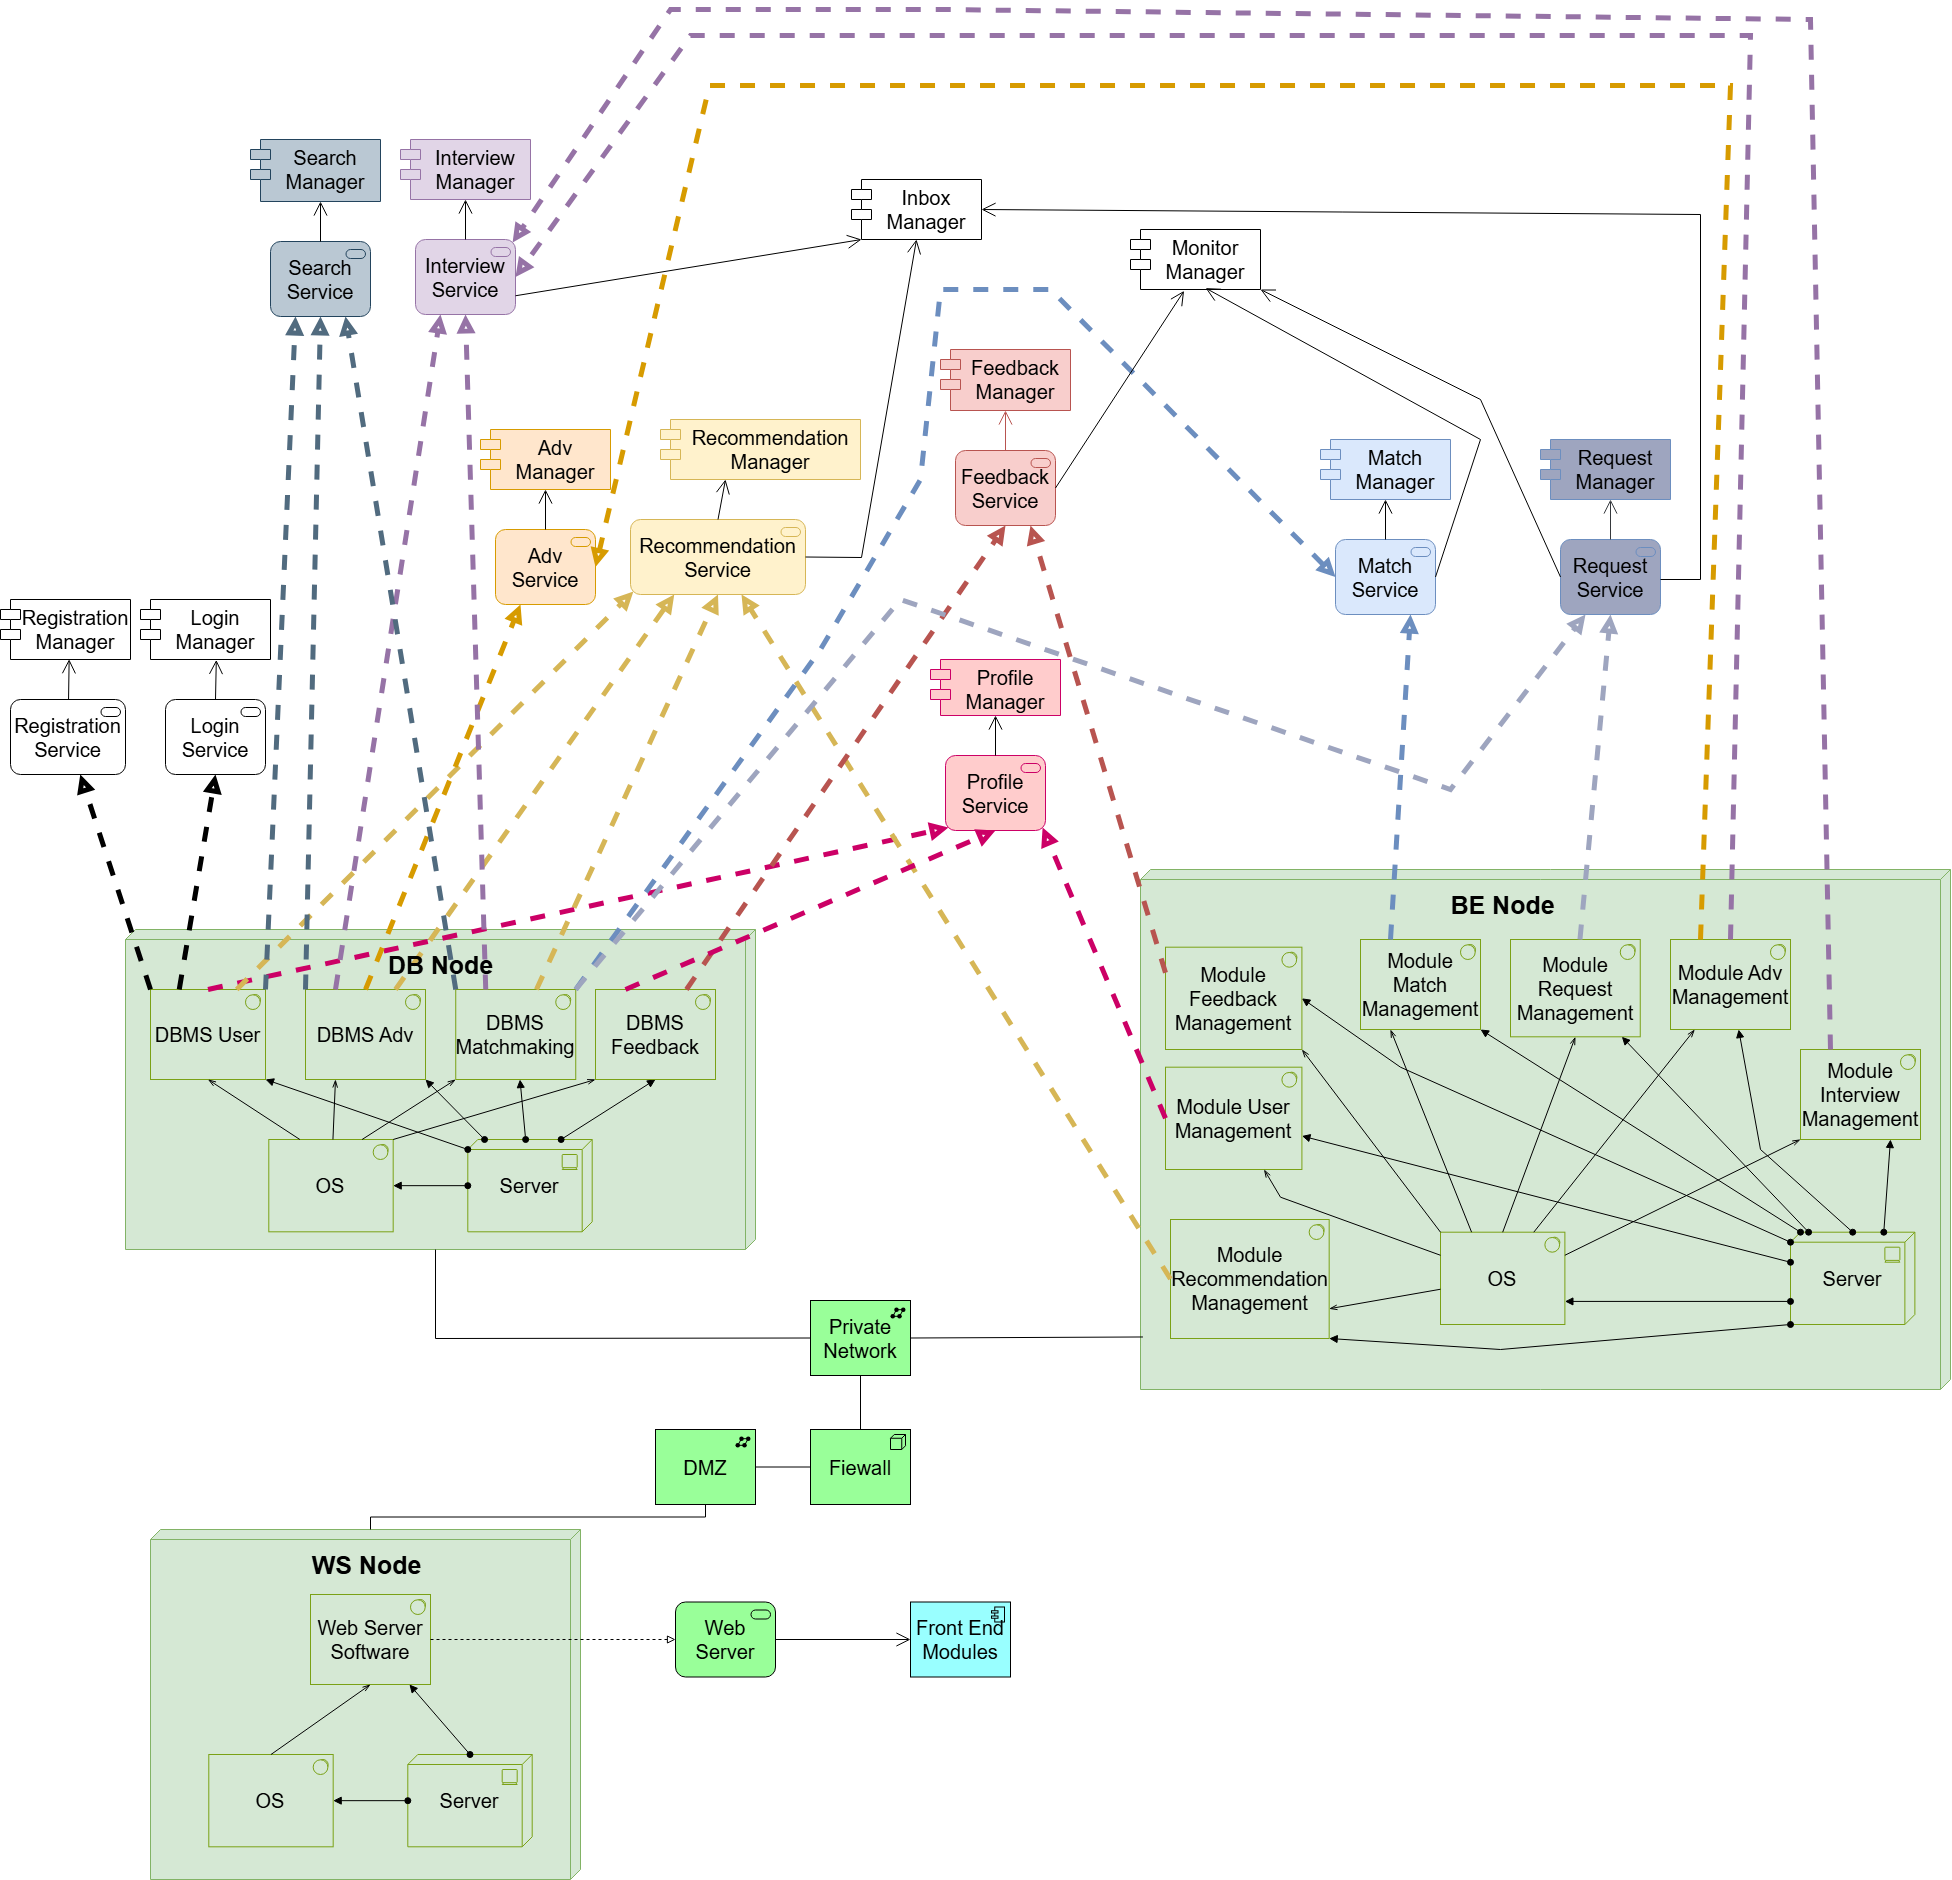
\includegraphics[width=15cm]{images/architectural design/deployment/DD-deploymentdiagram2.drawio.png}
    \caption{Deployment Diagram}
\end{figure}
This is an overview of the whole diagram, each node and module is going to be explained in detail with a zoomed image.
\subsection{Architecture nodes}
\begin{figure}[H]
    \centering
    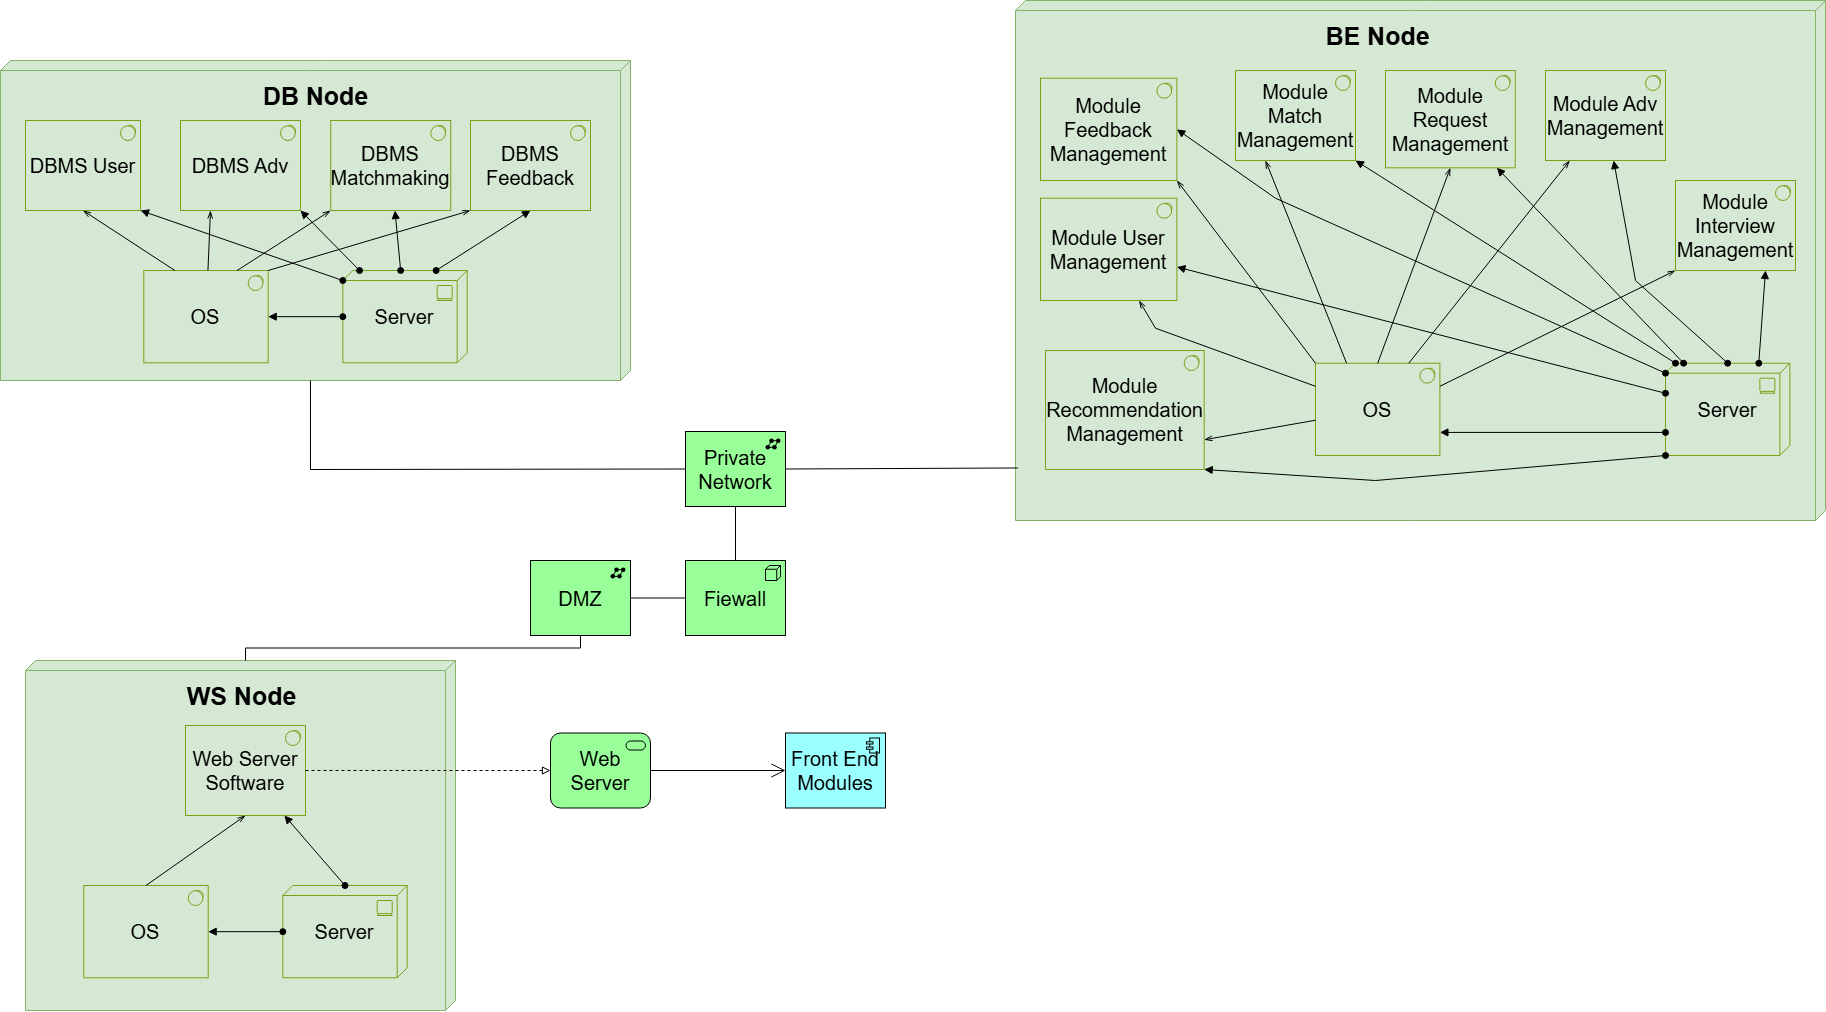
\includegraphics[width=15cm]{images/architectural design/deployment/depl-rete.drawio (1).png}
    \caption{Architecture nodes in Deployment Diagram}
\end{figure}
This is the architecture shown in the Overview Chapter, with the modules and components shown.
\subsubsection{Database Node}
\begin{figure}[H]
    \centering
    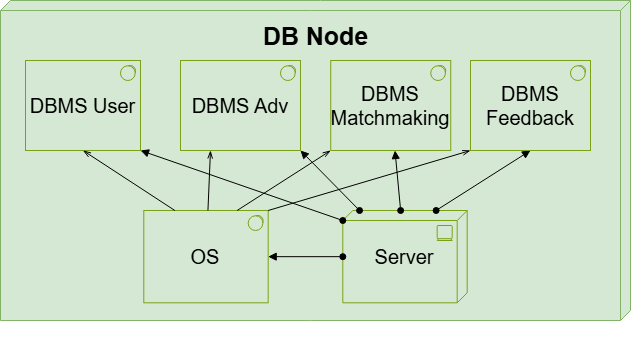
\includegraphics[width=15cm]{images/architectural design/deployment/depl-dbnode.drawio.png}
    \caption{Database Node in Deployment Diagram}
\end{figure}
This node is designed to centralise database management, it divides responsibilities across modules:
\begin{itemize}
    \item \textbf{User}: the DBs contain the information of both kinds of users, students, and companies.
    \item \textbf{Adv}: it organises the data of each internship advertisement, is related to the Company DB via external key.
    \item \textbf{Matchmaking}: it collects data about the matchmaking process: request messages, interview requests, matches' status.
    \item \textbf{Feedback}: feedback of companies and students is collected and connected to the respective user via external key.
\end{itemize}
The Operative System (OS) provides the base system for managing hardware and software resources on the DB Node and ensures the proper execution of database management systems and server processes. The Server facilitates communication between the DB Node and components.
\subsubsection{Back-End Node}
\begin{figure}[H]
    \centering
    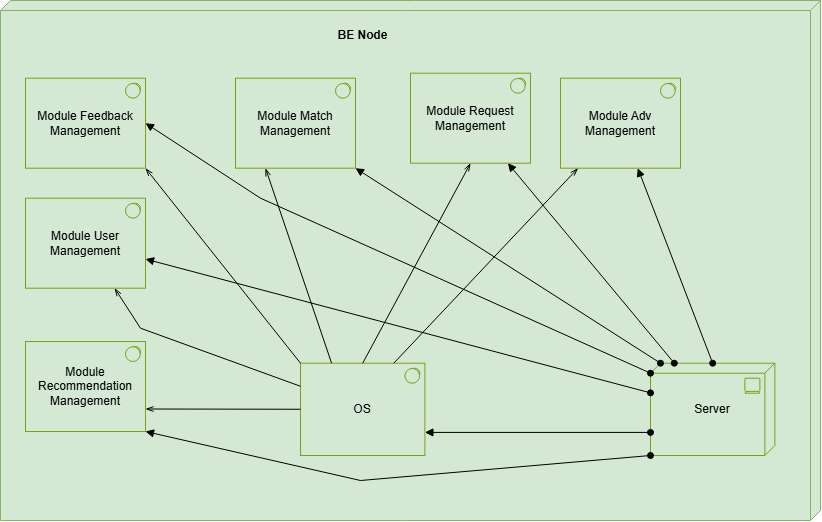
\includegraphics[width=15cm]{images/architectural design/deployment/depl-be.drawio.png}
    \caption{Back-End Node in Deployment Diagram}
\end{figure}
This node contains the business logic of the system, every module present runs specific functionalities related to the components, each module is seen in detail with the respective components and services. 
\subsection{Components and services}
\subsubsection{Sign up and Login}
\begin{figure}[H]
    \centering
    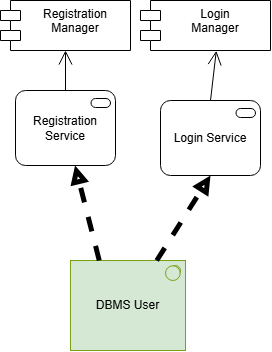
\includegraphics[width=0.25\linewidth]{images/architectural design/deployment/depl-login-signup.drawio.png}
    \caption{Deployment Diagram: Login and Sign up}
\end{figure}
Users sign up and logins are managed through database's query, so their services relies entirely on the User DBMS.
\subsubsection{Profile Management}
\begin{figure}[H]
    \centering
    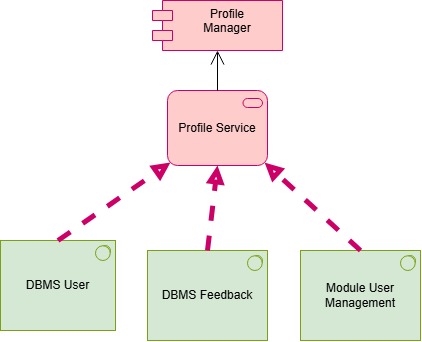
\includegraphics[width=0.40\linewidth]{images/architectural design/deployment/depl-profile.drawio.png}
    \caption{Deployment Diagram: Profile Management}
\end{figure}
Users' data is stored inside the DB so profiles are managed through queries to the DB and the functions inside the \textbf{Module Profile Manager}.

\subsubsection{ADV Management}
\begin{figure}[H]
    \centering
    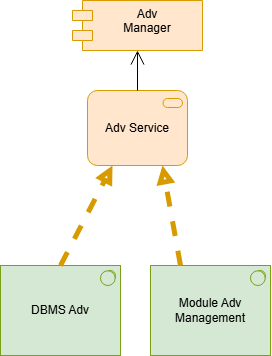
\includegraphics[width=0.25\linewidth]{images/architectural design/deployment/deply-adv.drawio.png}
    \caption{Deployment Diagram: ADV Management}
\end{figure}
ADV's data is stored inside the DB, while the functions to manage them are found in the \textbf{Manage ADV Module}.

\subsubsection{Interview Management}
\begin{figure}[H]
    \centering
    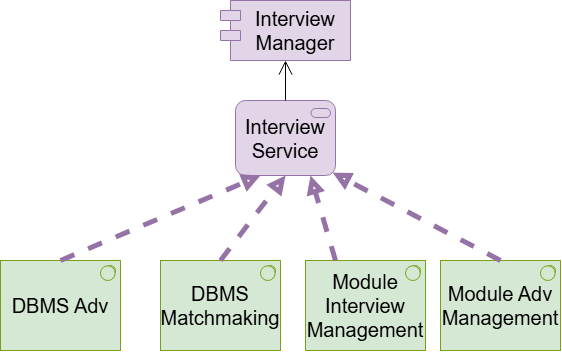
\includegraphics[width=0.45\linewidth]{images/architectural design/deployment/depl-inter.drawio.png}
    \caption{Deployment Diagram: Interview Management}
\end{figure}
Interview Manager handles interview forms and interview requests. Interview forms are stored in the \textbf{Adv DBMS} and managed by both \textbf{Module Adv Management} and \textbf{Module Interview Manager}, while interview requests are stored inside the \textbf{Matchmaking DBMS} and managed by the \textbf{Module Interview Management}.

\subsubsection{Search Management}
\begin{figure}[H]
    \centering
    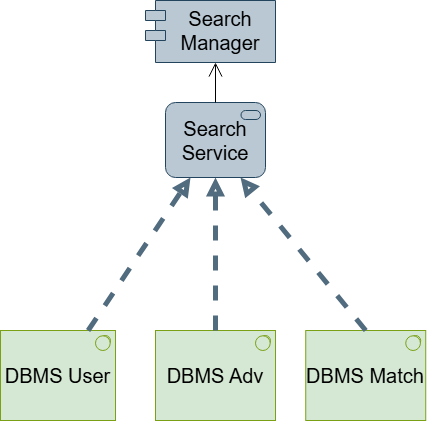
\includegraphics[width=0.25\linewidth]{images/architectural design/deployment/depl-search.drawio (1).png}
    \caption{Deployment Diagram: Search Management}
\end{figure}
User searches rely on the Users DB and on the ADV, they are managed through queries. Also, the fields inserted by the students are stored inside the correspondent DB (in the User DBMS) in order to make proper recommendations. The search results cannot be already matched with the user searching, so the results are checked with the matches inside the DB.

\subsubsection{Recommendation Management}
\begin{figure}[H]
    \centering
    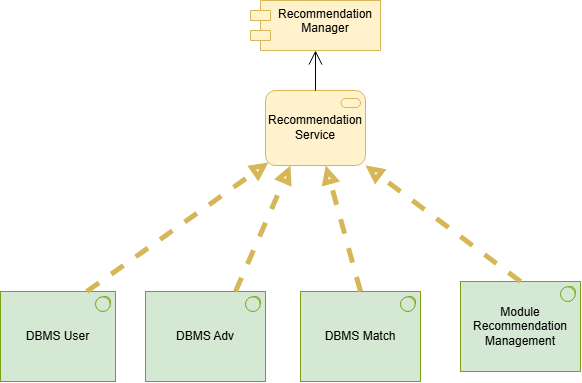
\includegraphics[width=0.45\linewidth]{images/architectural design/deployment/depl-recc.drawio.png}
    \caption{Deployment Diagram: Recommendation Management}
\end{figure}
Recommendations are based on Users and ADVs, so they are based on the data in the DBs and managed through the functions in the \textbf{Recommendation Manager}. They can also queries the Matchmaking DBMS to make sure that the recommended profiles are not already matched. 

\subsubsection{Match Management}
\begin{figure}[H]
    \centering
    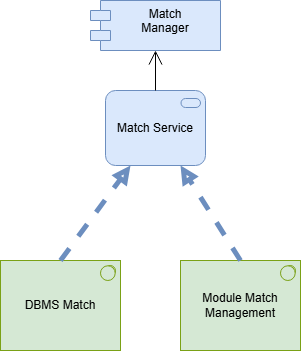
\includegraphics[width=0.25\linewidth]{images/architectural design/deployment/depl-match.drawio.png}
    \caption{Deployment Diagram: Match Management}
\end{figure}
Matches are stored in the DB and are managed through the functions of \textbf{Module Match Management}.

\subsubsection{Feedback Management}
\begin{figure}[H]
    \centering
    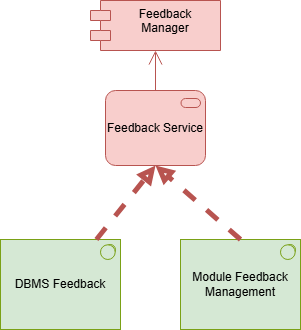
\includegraphics[width=0.25\linewidth]{images/architectural design/deployment/depl-feed.drawio.png}
    \caption{Deployment Diagram: Feedback Management}
\end{figure}
Feedbacks are stored inside the DB and are managed through the \textbf{Module Feedback Management}.

\subsubsection{Monitor and Inbox Management}
\begin{figure}[H]
    \centering
    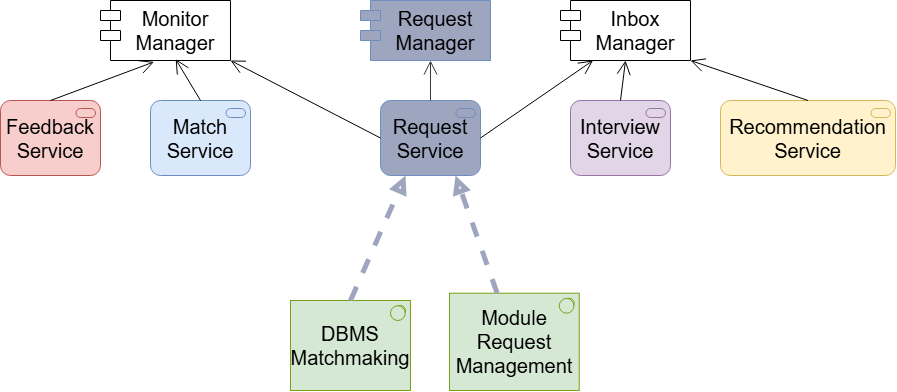
\includegraphics[width=0.65\linewidth]{images/architectural design/deployment/depl-requ.drawio.png}
    \caption{Deployment Diagram: Monitor and Inbox Management}
\end{figure}
The Monitor Section shows the user's matches, and it is where users can leave feedbacks, so it is based on the \textbf{Match Service}, the \textbf{Request Service}, and the \textbf{Feedback Service}.
The Inbox Section shows match and interview requests, and recommendations sent to the user, so it is based on the \textbf{Request Service} that is managed through the \textbf{Module Request Manager}, the \textbf{Recommendation Service}, and the \textbf{Interview Serivce}. 
\section{Runtime view}
\begin{figure}[H]
\textbf{Student Sign up}\newline\newline
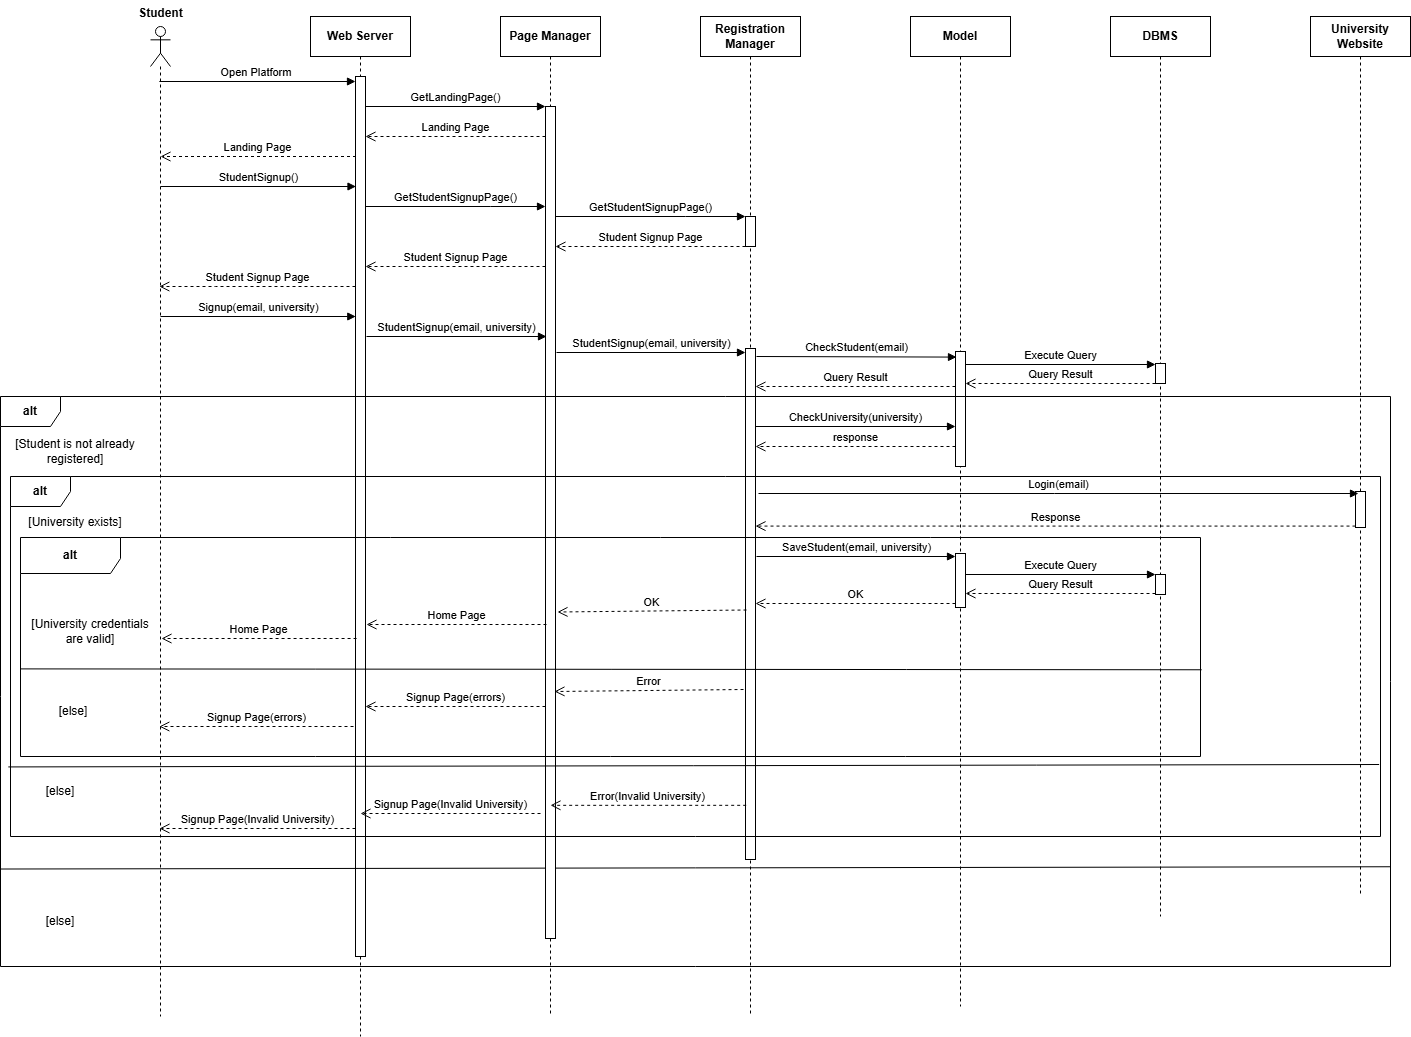
\includegraphics[width=15cm]{images/architectural design/runtime/DD-UC1.drawio (1).png}
    \caption{SD: Student Sign up}
\end{figure}

\begin{figure}[H]
\textbf{Student Login}\newline\newline
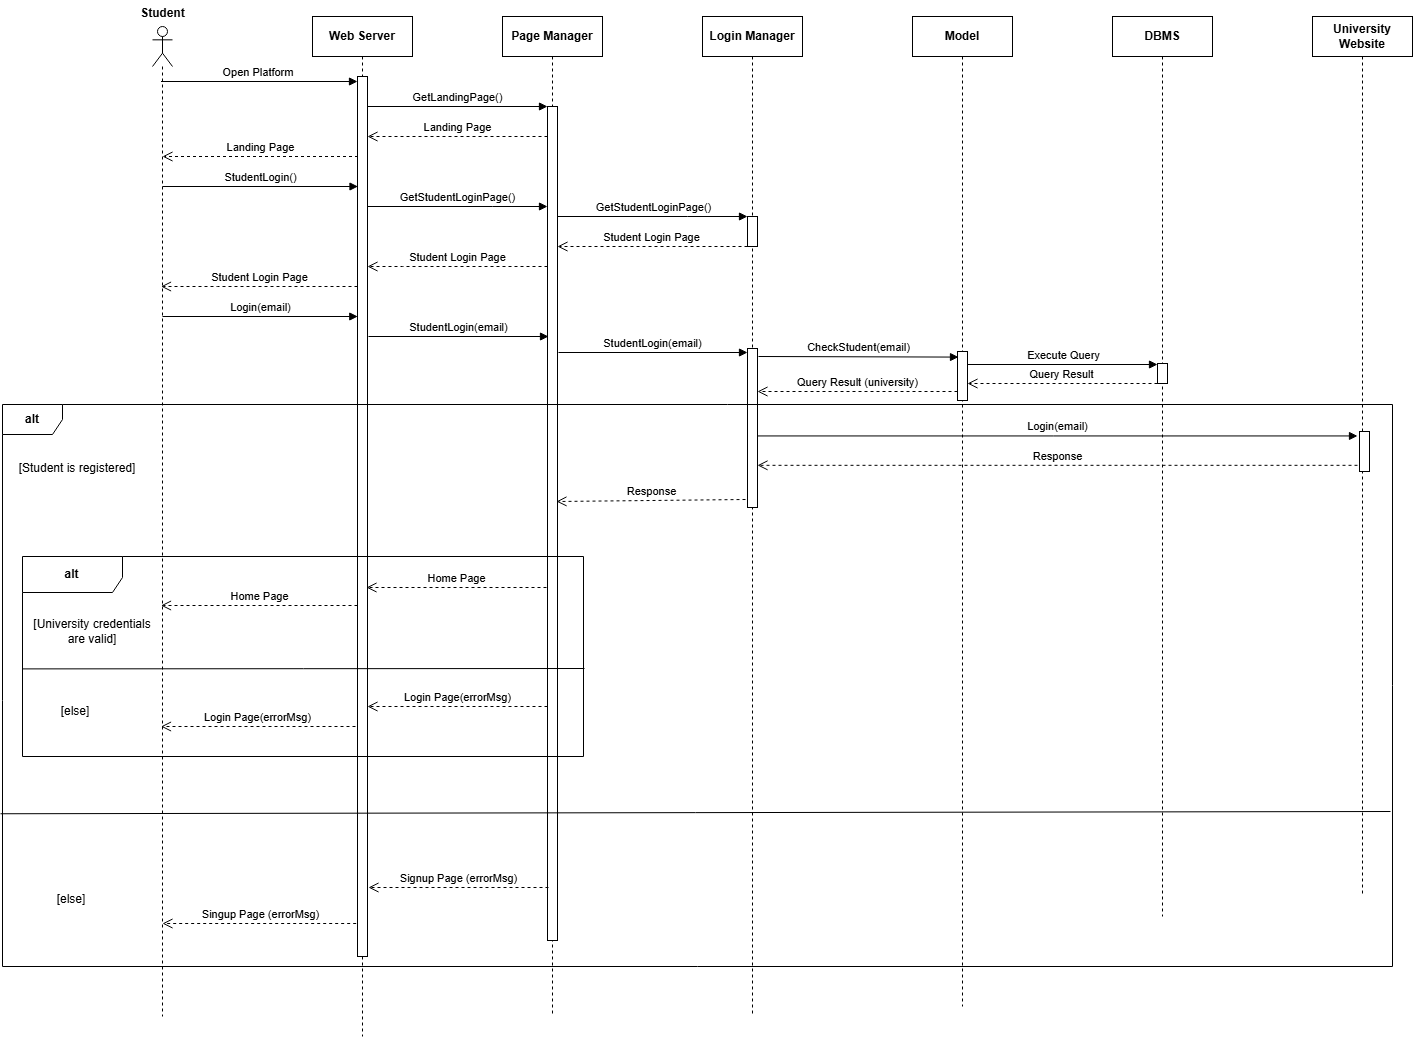
\includegraphics[width=15cm]{images/architectural design/runtime/DD-UC2.drawio.png}
    \caption{SD: Student Login}
\end{figure}

\begin{figure}[H]
\textbf{Company Sign up}\newline\newline
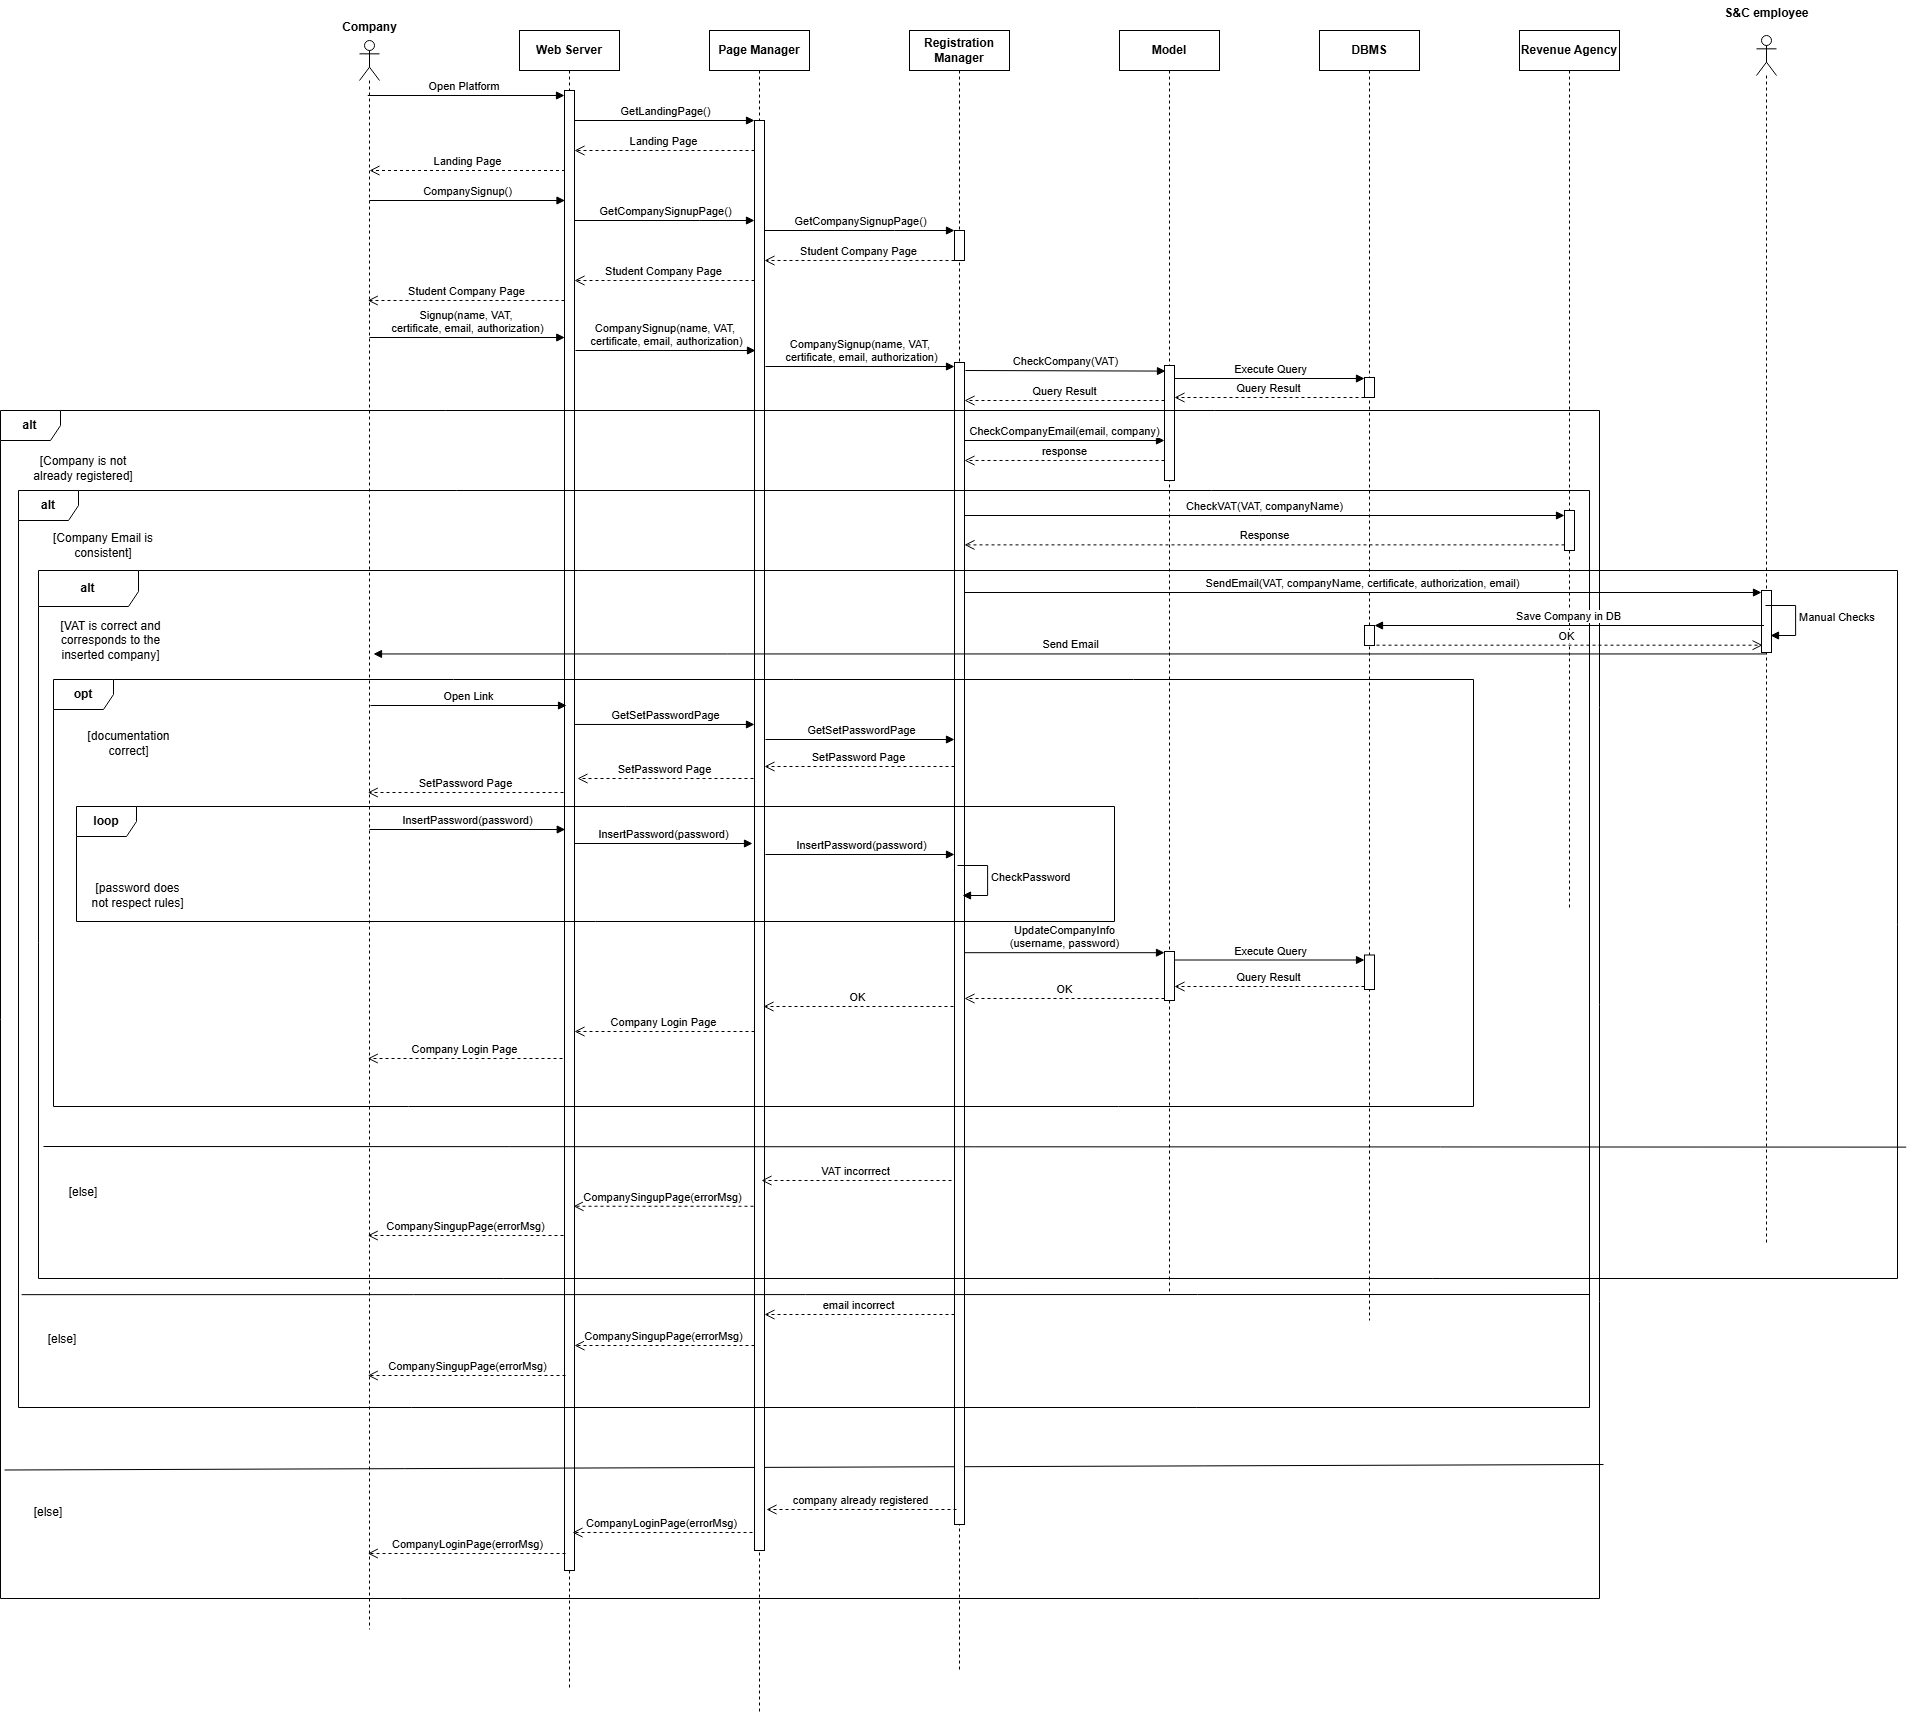
\includegraphics[width=15cm]{images/architectural design/runtime/DD-UC3.drawio.png}
    \caption{SD: Company Sign up}
\end{figure}

\begin{figure}[H]
\textbf{Company Login}\newline\newline
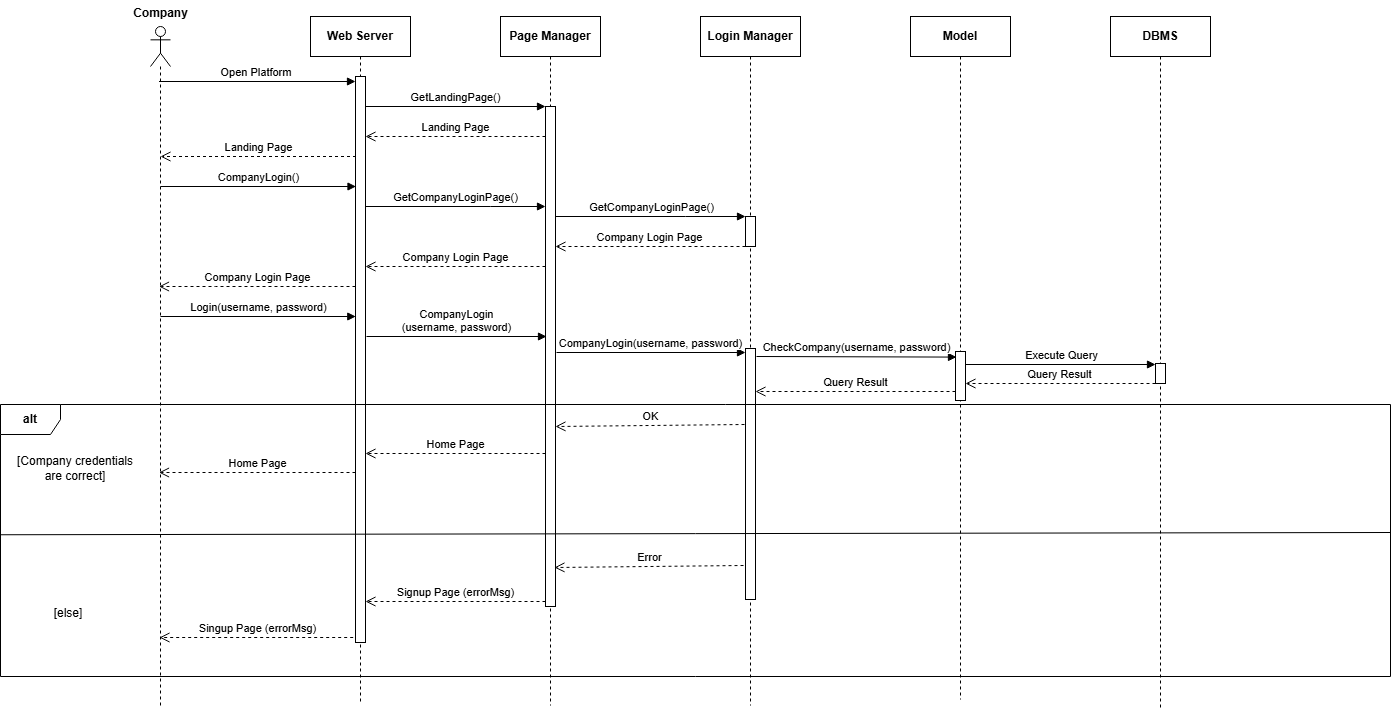
\includegraphics[width=15cm]{images/architectural design/runtime/DD-UC4.drawio.png}
    \caption{SD: Company Login}
\end{figure}

\begin{figure}[H]
\textbf{Upload Student CV}\newline\newline
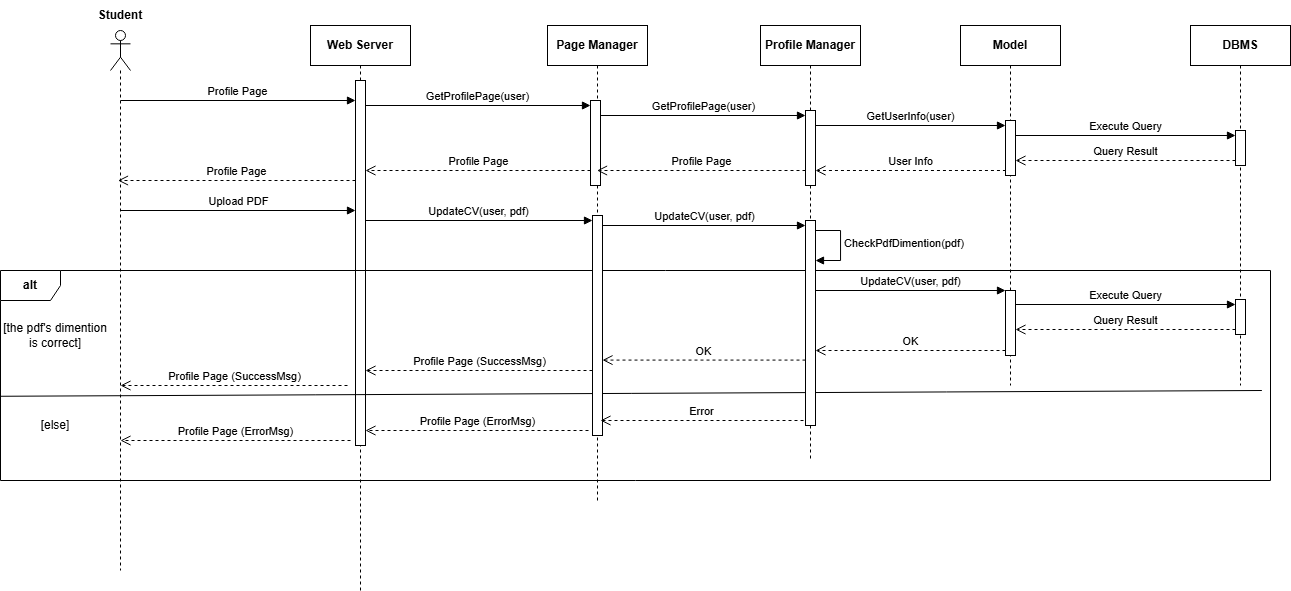
\includegraphics[width=15cm]{images/architectural design/runtime/DD-UC5.drawio.png}
    \caption{SD: Upload Student CV}
\end{figure}

\begin{figure}[H]
\textbf{Add new competence}\newline\newline
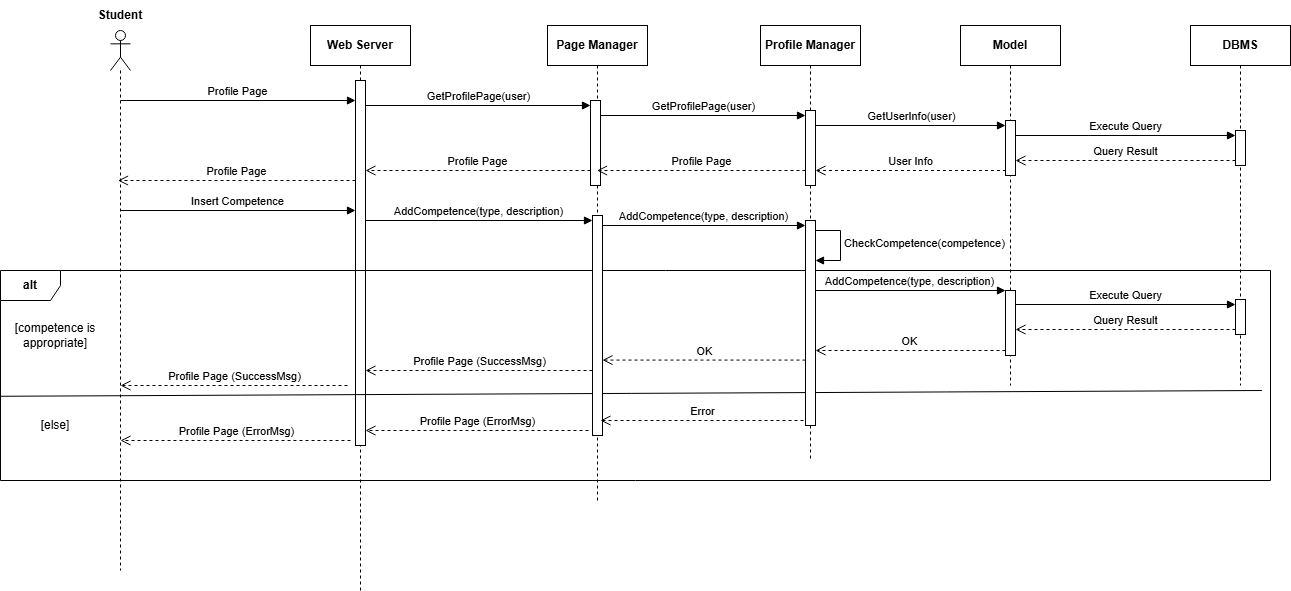
\includegraphics[width=15cm]{images/architectural design/runtime/DD-UC6.drawio.png}
    \caption{SD: Add new competence}
\end{figure}

\begin{figure}[H]
\textbf{Edit competence}\newline\newline
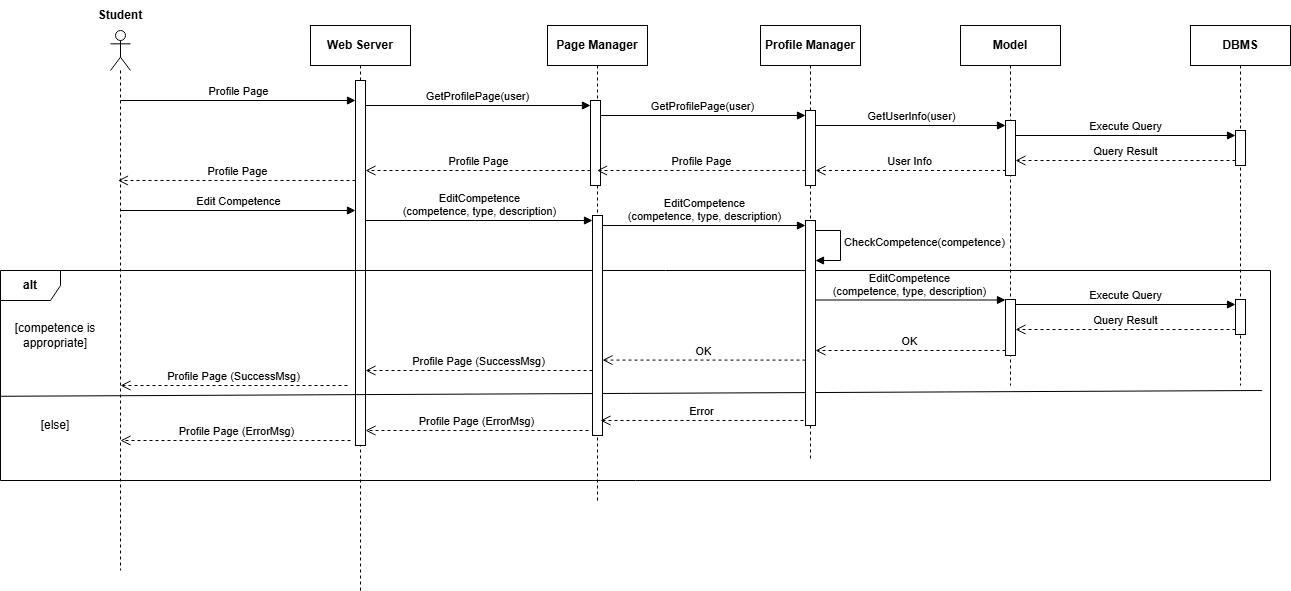
\includegraphics[width=15cm]{images/architectural design/runtime/DD-UC7.drawio.png}
    \caption{SD: Edit competence}
\end{figure}

\begin{figure}[H]
\textbf{Create New ADV}\newline\newline
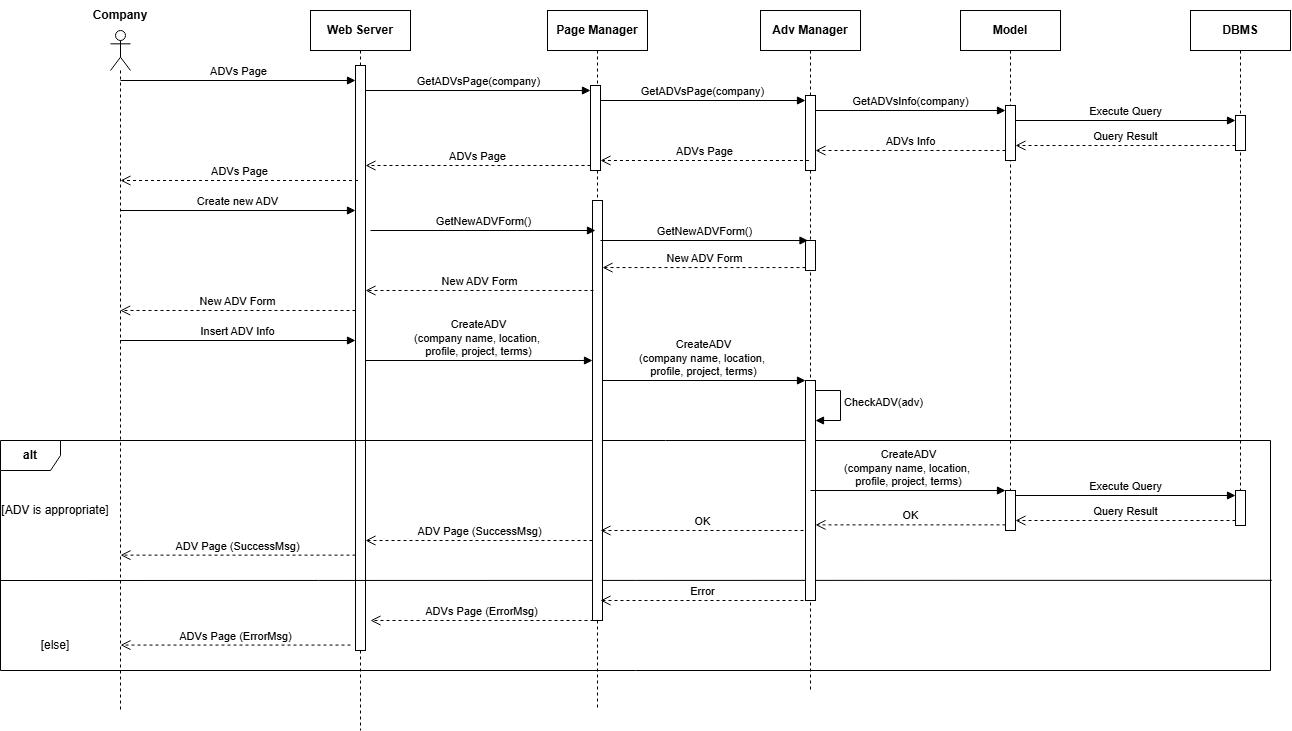
\includegraphics[width=15cm]{images/architectural design/runtime/DD-UC8.drawio (1).png}
    \caption{SD: Create New ADV}
\end{figure}

\begin{figure}[H]
\textbf{Edit ADV}\newline\newline
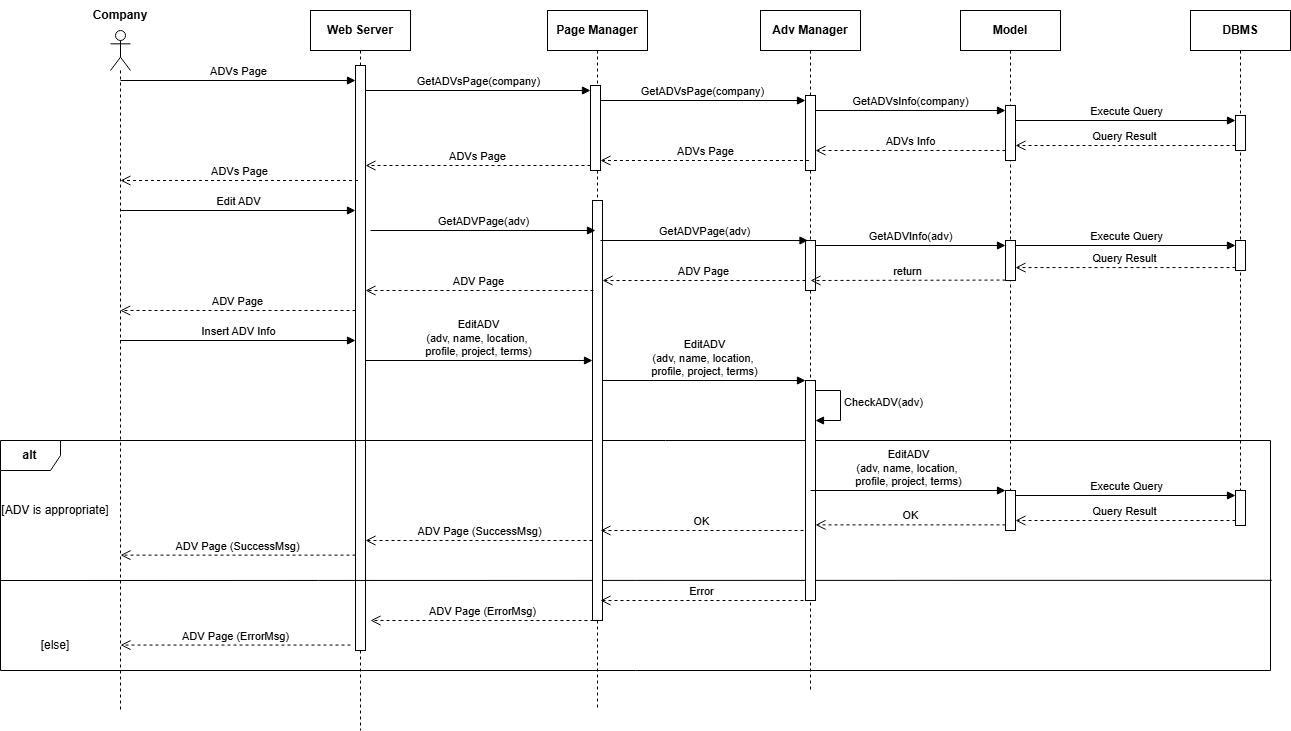
\includegraphics[width=15cm]{images/architectural design/runtime/DD-UC9.drawio (1).png}
    \caption{SD: Edit ADV}
\end{figure}

\begin{figure}[H]
\textbf{Delete ADV}\newline\newline
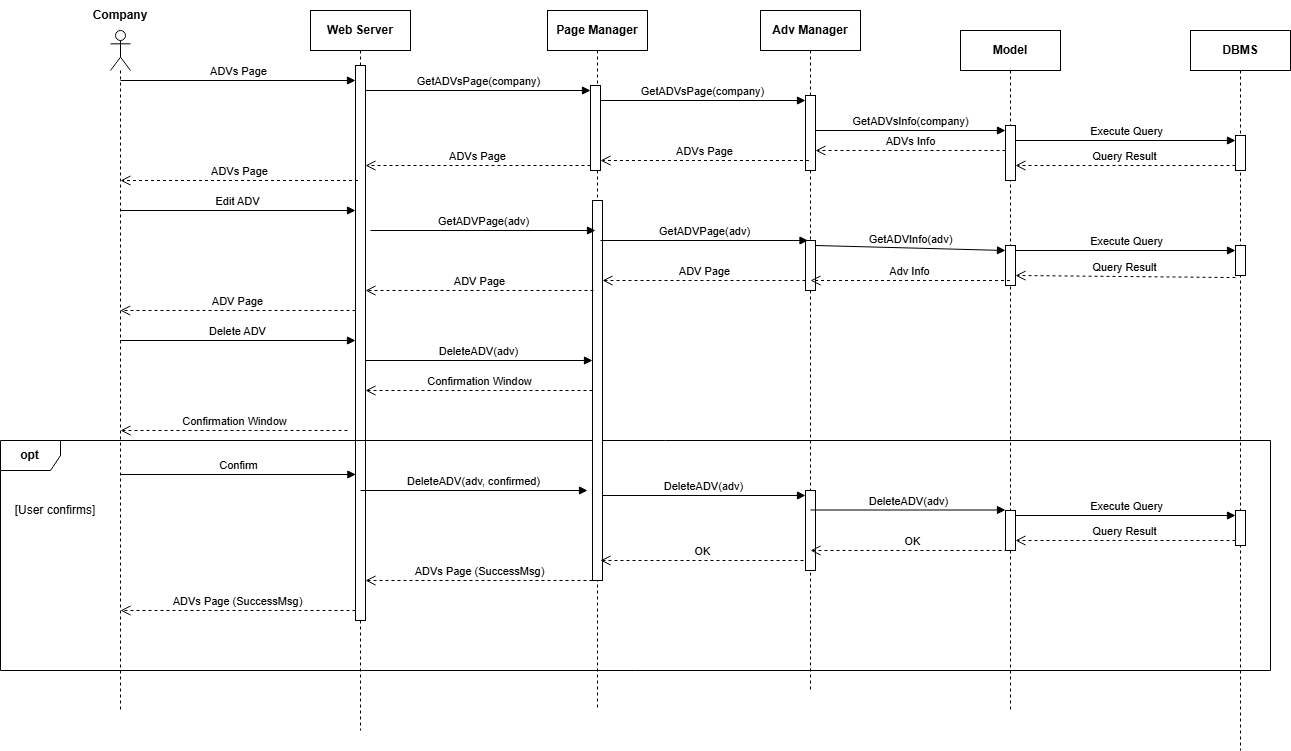
\includegraphics[width=15cm]{images/architectural design/runtime/DD-UC10.drawio (1).png}
    \caption{SD: Delete ADV}
\end{figure}

\begin{figure}[H]
\textbf{Proactive Internship Search}\newline\newline
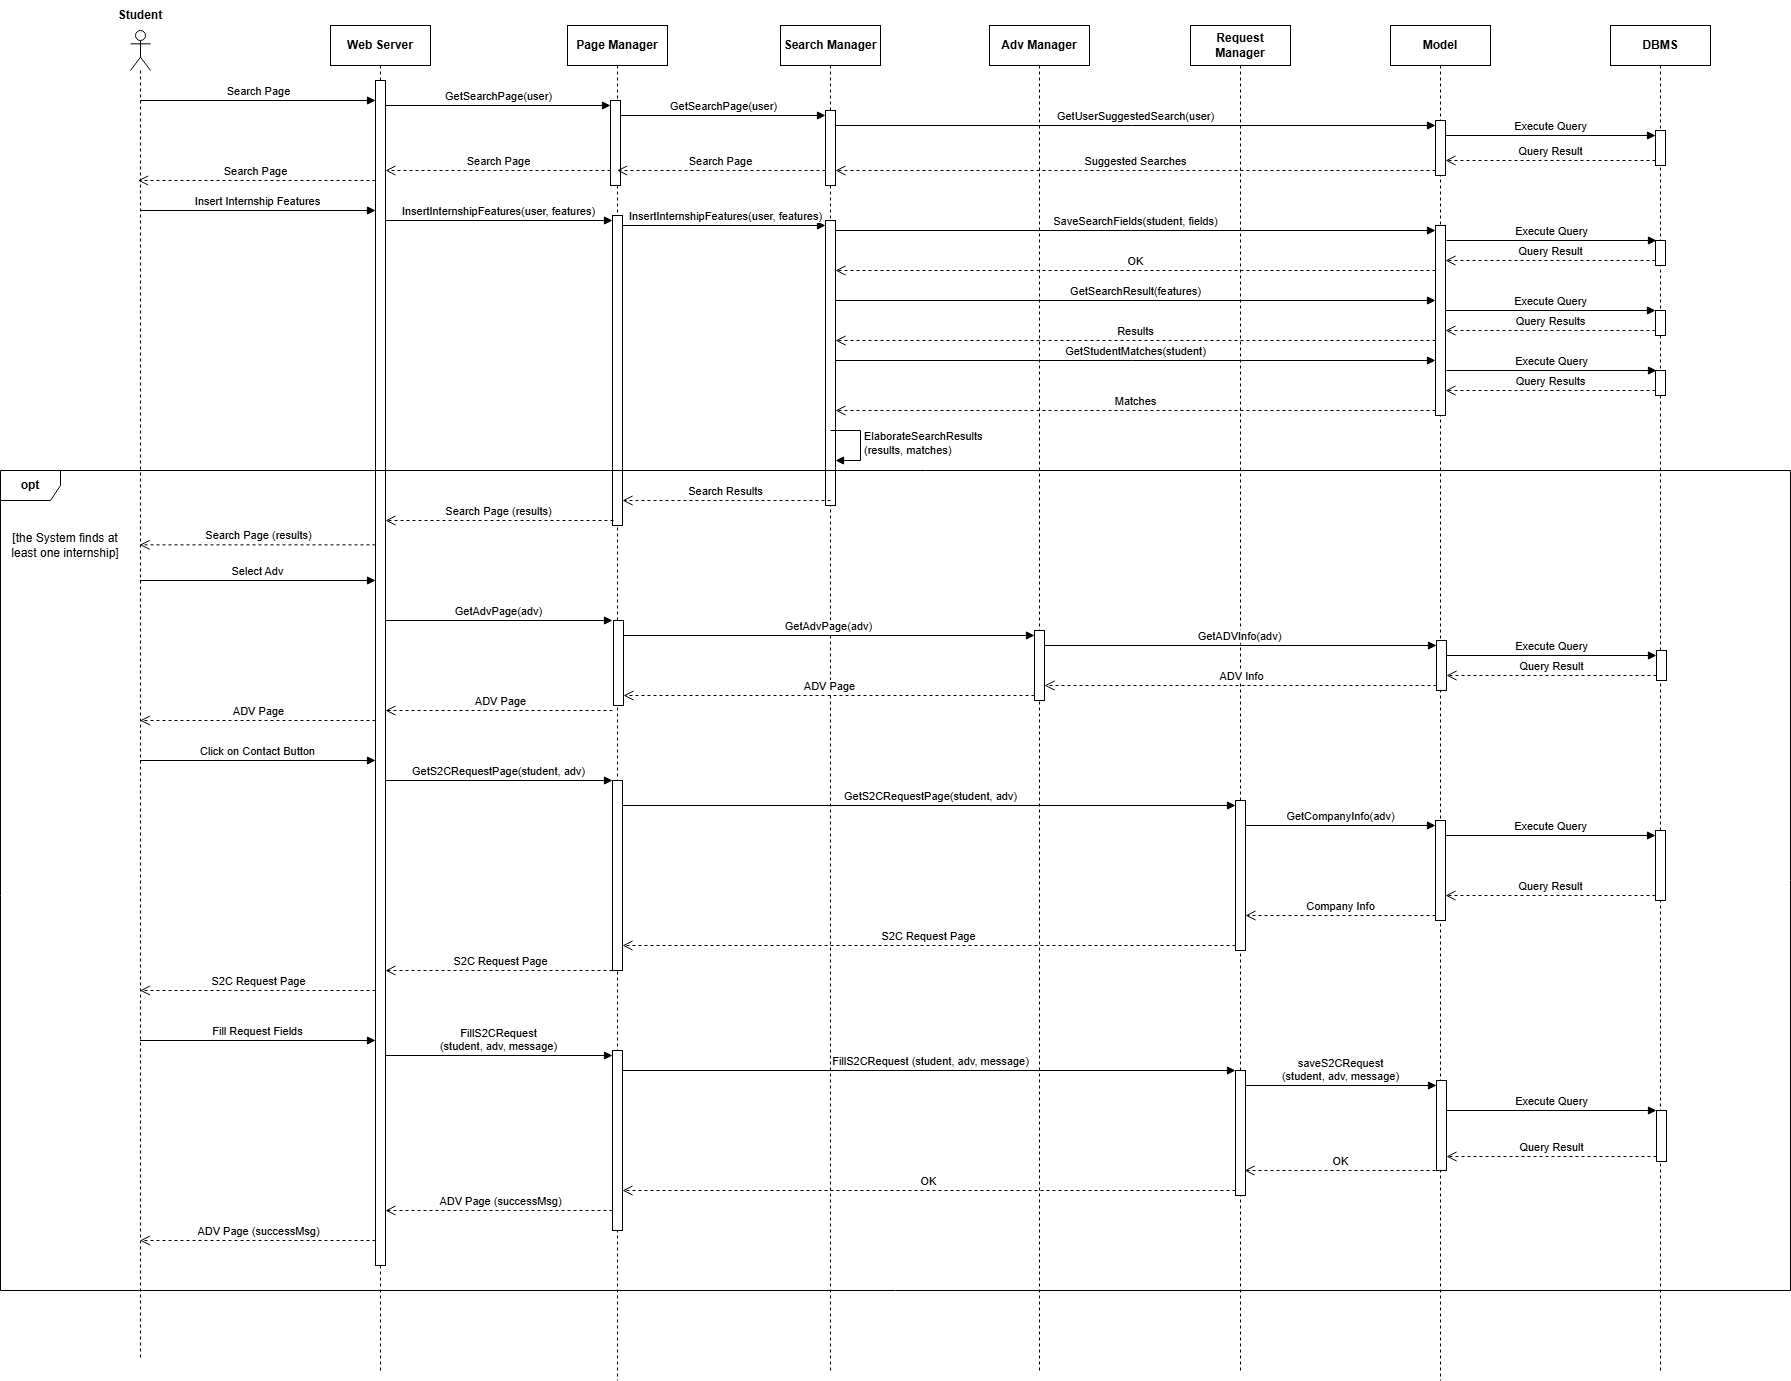
\includegraphics[width=15cm]{images/architectural design/runtime/DD-UC11.drawio.png}
    \caption{SD: Proactive Internship Search}
\end{figure}

\begin{figure}[H]
\textbf{Proactive Candidate Search}\newline\newline
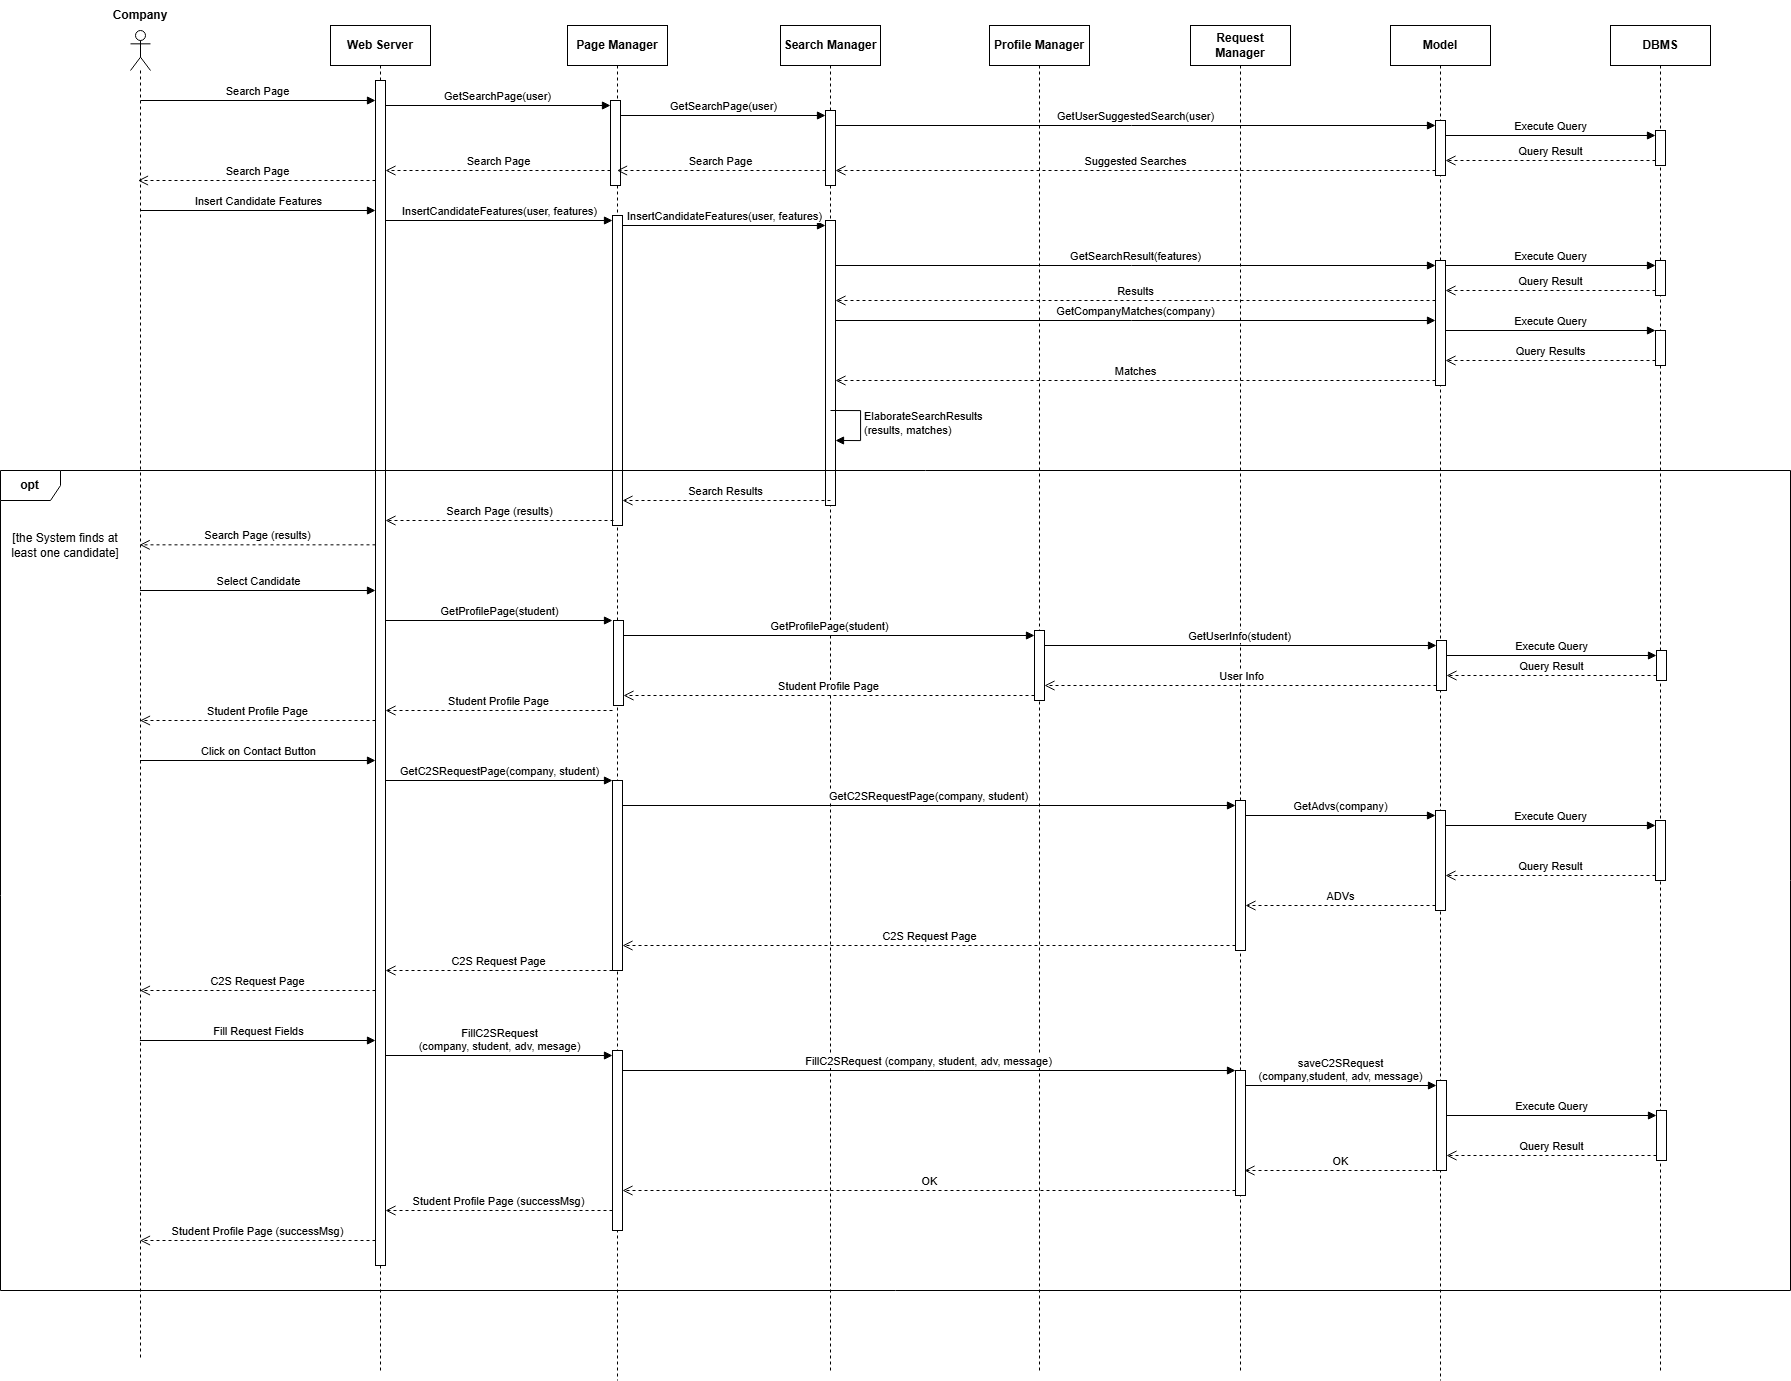
\includegraphics[width=15cm]{images/architectural design/runtime/DD-UC12.drawio.png}
    \caption{SD: Proactive Candidate Search}
\end{figure}

\begin{figure}[H]
\textbf{Recommendation}\newline\newline
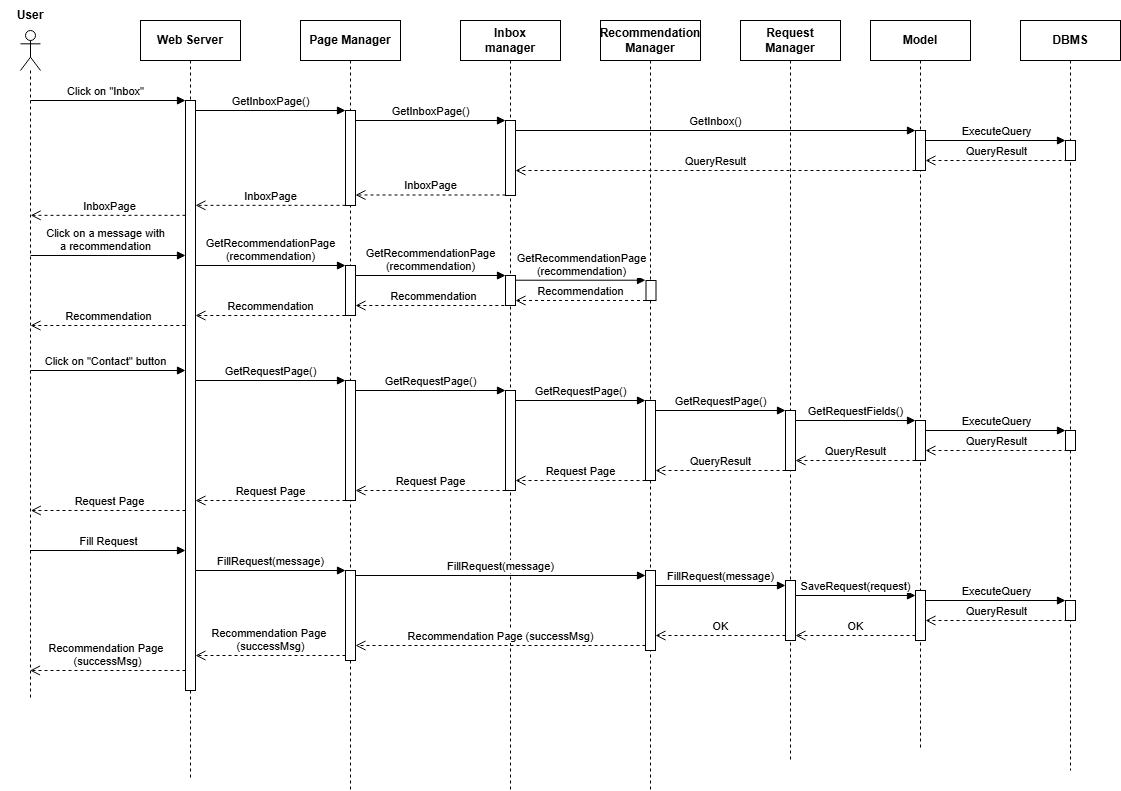
\includegraphics[width=15cm]{images/architectural design/runtime/DD-UC13.drawio.png}
    \caption{SD: Recommendation}
\end{figure}
\textit{Note}: This diagram is generalised for every type of user, so the request's functions are generalised too. The specific ones are used in the search diagrams.

\begin{figure}[H]
\textbf{Accept internship request (Student)}\newline\newline
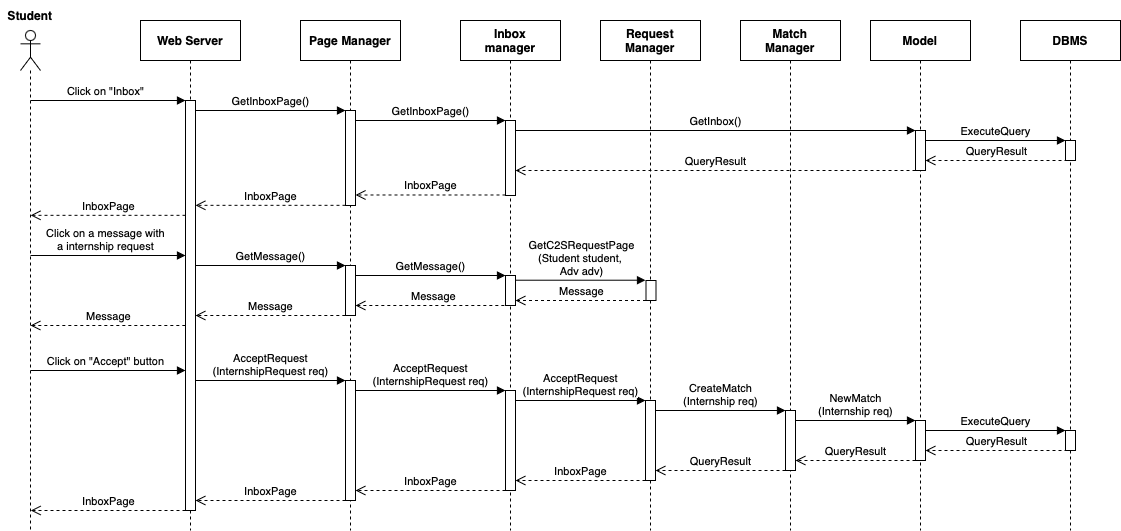
\includegraphics[width=15cm]{images/architectural design/runtime/DD-UC16.1.drawio.png}
    \caption{SD: Accept internship request (Student)}
\end{figure}

\begin{figure}[H]
\textbf{Reject internship request (Student)}\newline\newline
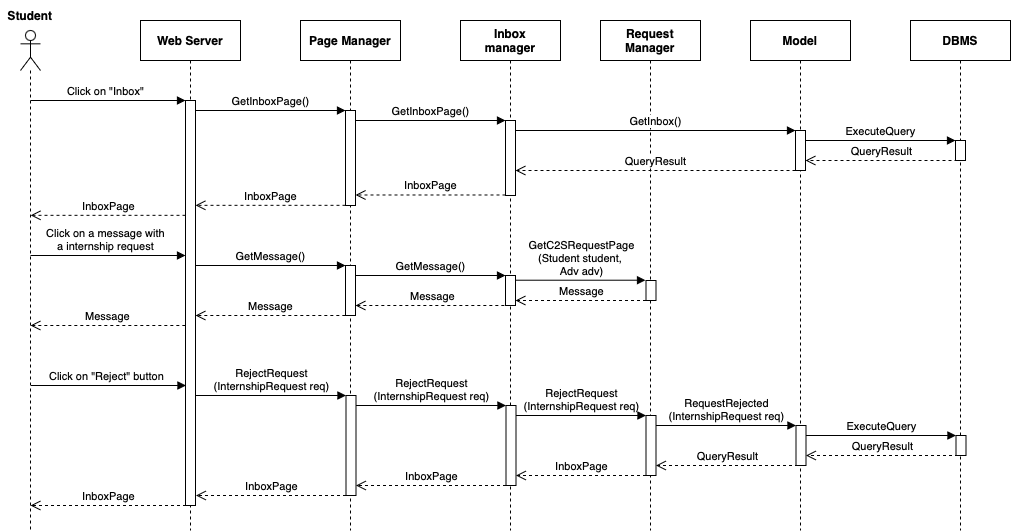
\includegraphics[width=15cm]{images/architectural design/runtime/DD-UC16.2.drawio.png}
    \caption{SD: Reject internship request (Student)}
\end{figure}

\begin{figure}[H]
\textbf{Accept internship request (Company)}\newline\newline
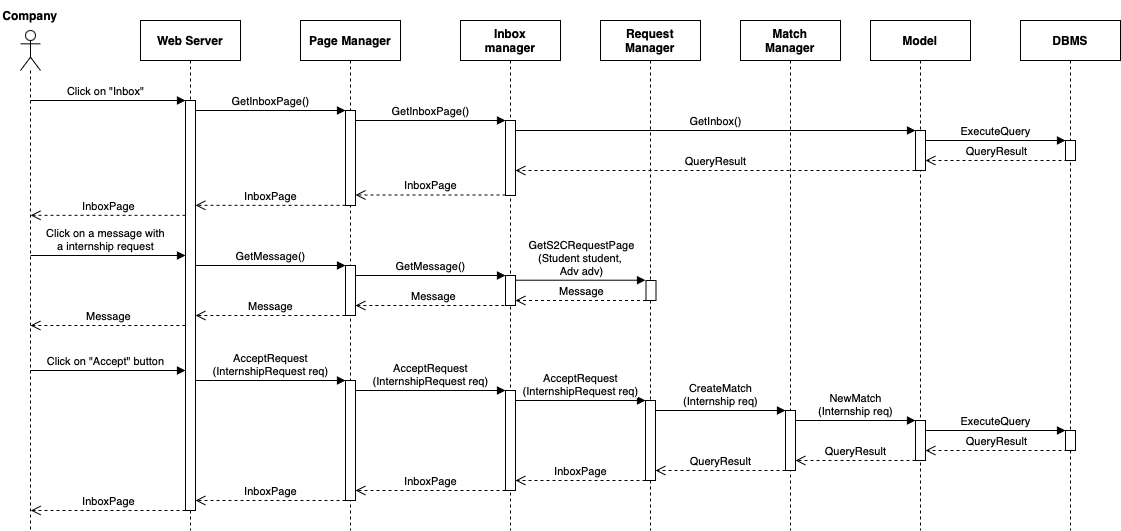
\includegraphics[width=15cm]{images/architectural design/runtime/DD-UC17.1.drawio.png}
    \caption{SD: Accept internship request (Company)}
\end{figure}

\begin{figure}[H]
\textbf{Reject internship request (Company)}\newline\newline
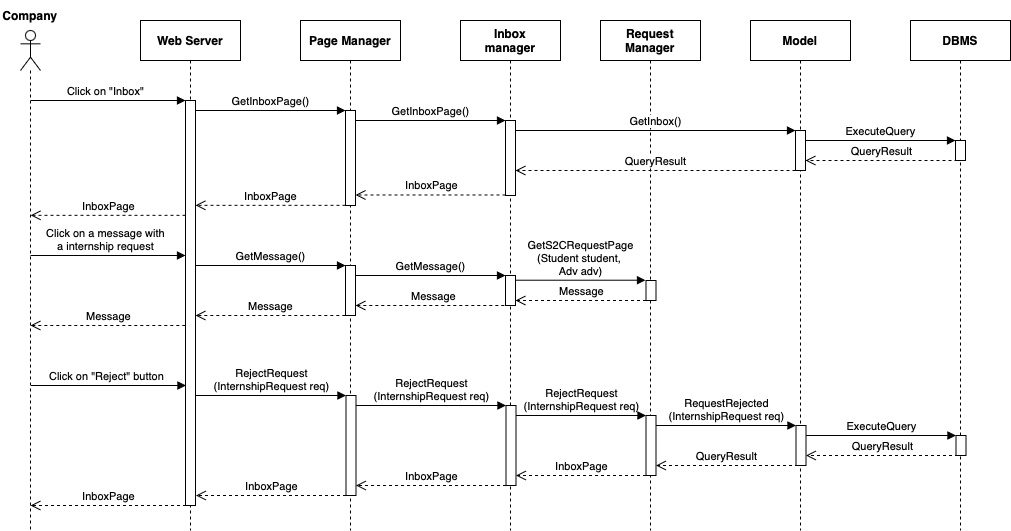
\includegraphics[width=15cm]{images/architectural design/runtime/DD-UC17.2.drawio.png}
    \caption{SD: Reject internship request (Company)}
\end{figure}

\begin{figure}[H]
\textbf{Check request outcome (Student)}\newline\newline
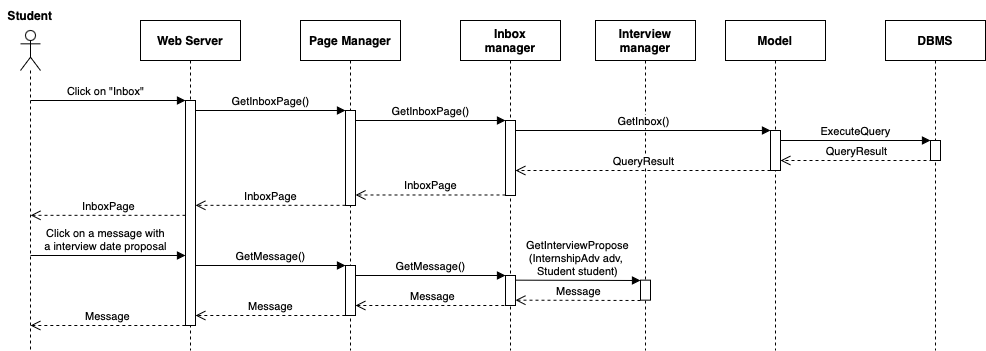
\includegraphics[width=15cm]{images/architectural design/runtime/DD-UC18.drawio.png}
    \caption{SD: Check request outcome (Student)}
\end{figure}

\begin{figure}[H]
\textbf{Check request outcome (Company)}\newline\newline
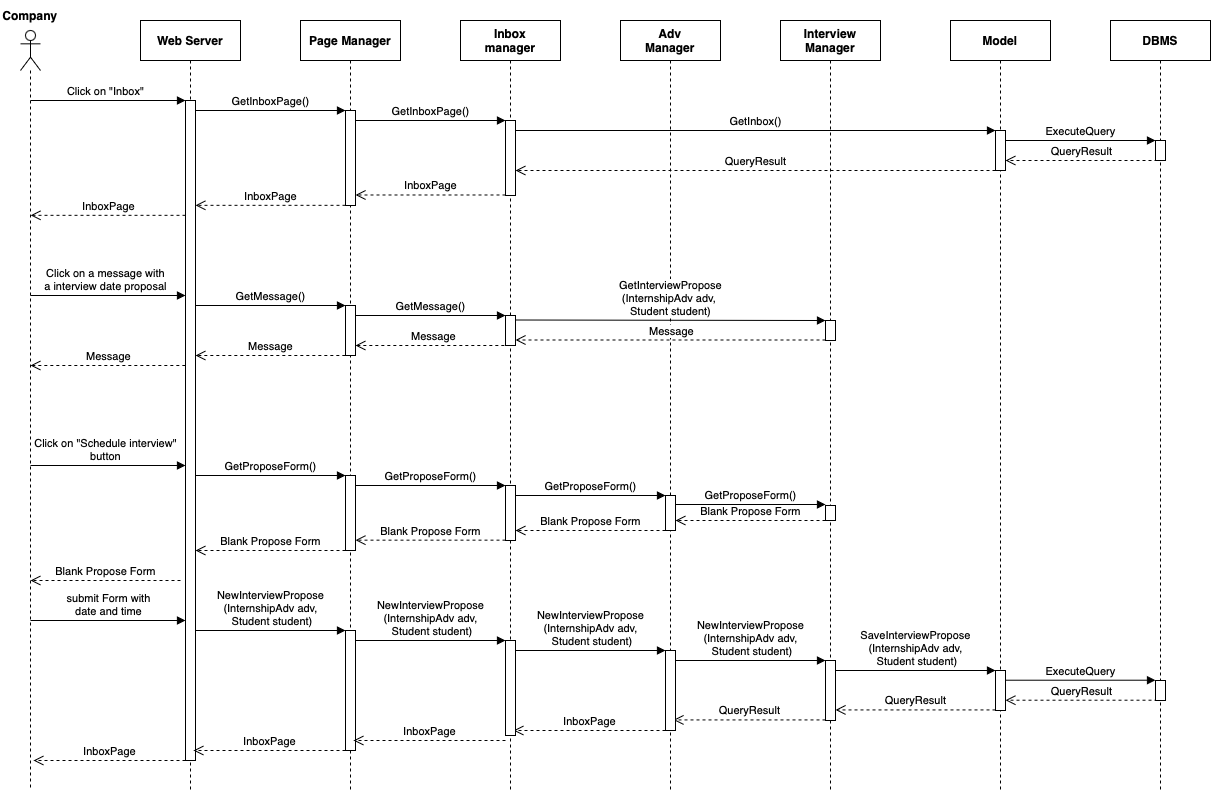
\includegraphics[width=15cm]{images/architectural design/runtime/DD-UC19.drawio.png}
    \caption{SD: Check request outcome (Company)}
\end{figure}

\begin{figure}[H]
\textbf{Propose a date for an interview}\newline\newline
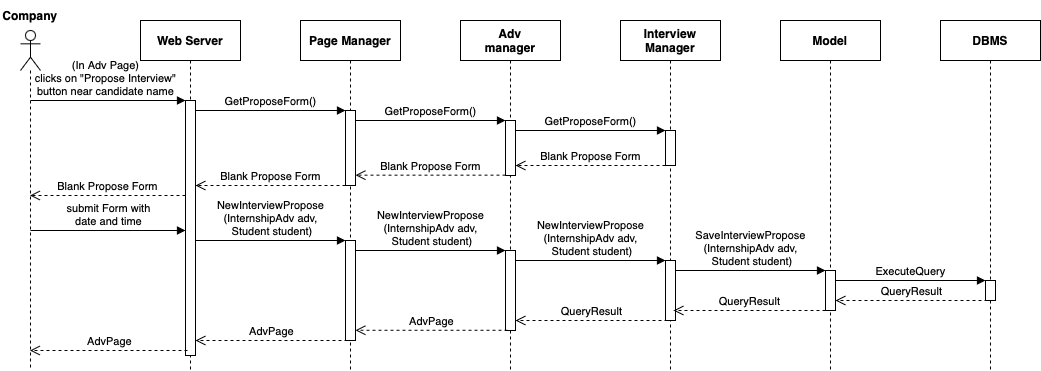
\includegraphics[width=15cm]{images/architectural design/runtime/DD-UC20.1.drawio.png}
    \caption{SD: Propose a date for an interview}
\end{figure}

\begin{figure}[H]
\textbf{Accept a date for an interview}\newline\newline
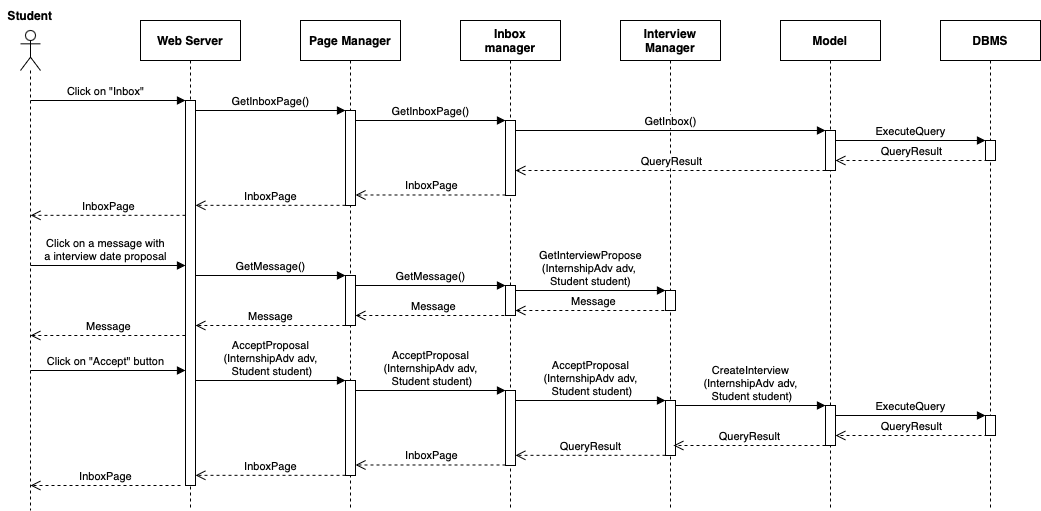
\includegraphics[width=15cm]{images/architectural design/runtime/DD-UC20.2.drawio.png}
    \caption{SD: Accept a date for an interview}
\end{figure}

\begin{figure}[H]
\textbf{Reject a date for an interview}\newline\newline
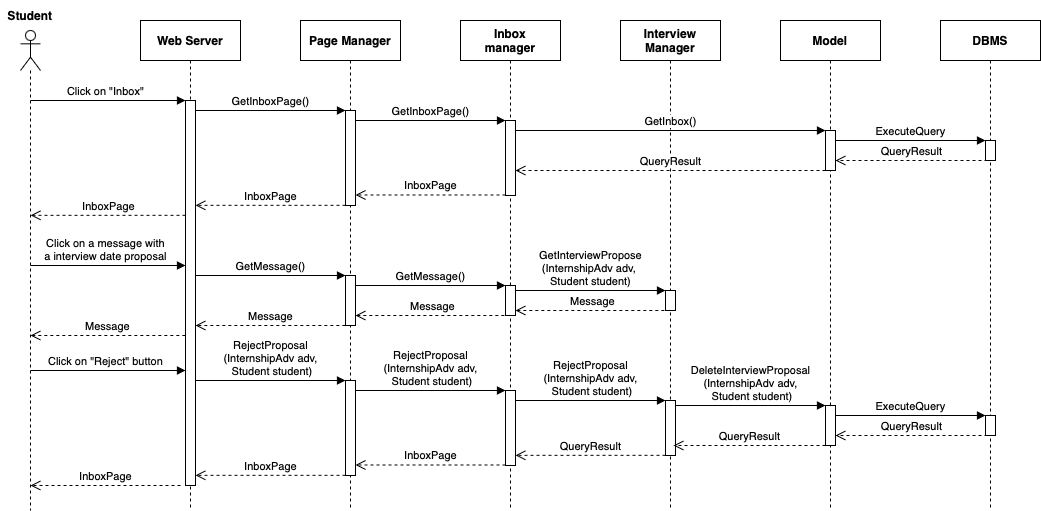
\includegraphics[width=15cm]{images/architectural design/runtime/DD-UC20.3.drawio.png}
    \caption{SD: Reject a date for an interview}
\end{figure}

\begin{figure}[H]
\textbf{Creating form for interview}\newline\newline
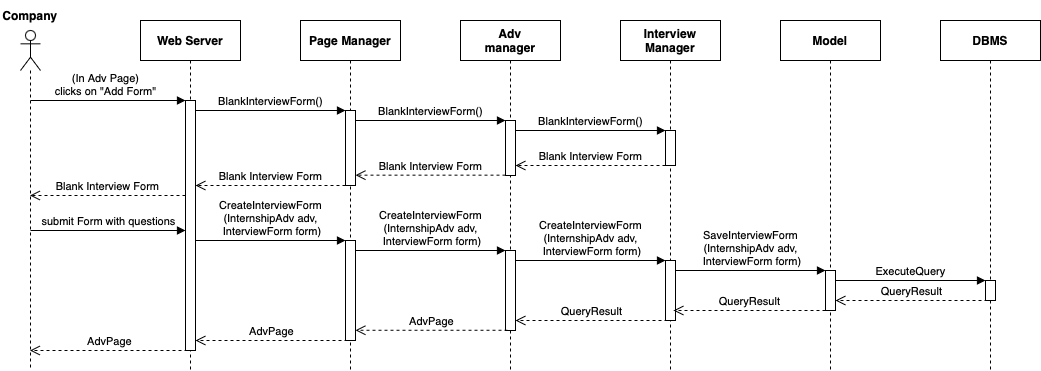
\includegraphics[width=15cm]{images/architectural design/runtime/DD-UC21.drawio.png}
    \caption{SD: Creating form for interview}
\end{figure}

\begin{figure}[H]
\textbf{Deleting form for interview}\newline\newline
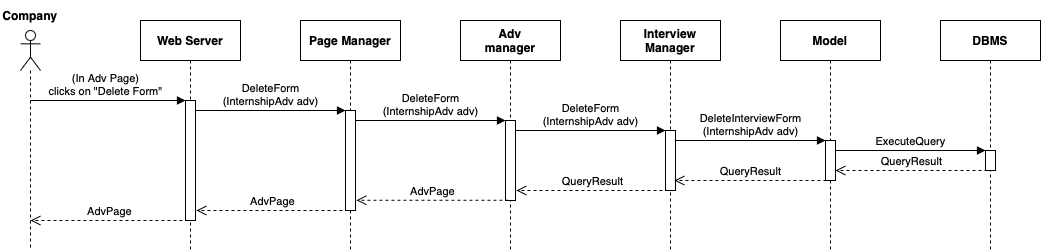
\includegraphics[width=15cm]{images/architectural design/runtime/DD-UC22.1.drawio.png}
    \caption{SD: Deleting form for interview}
\end{figure}

\begin{figure}[H]
\textbf{Modify form for interview}\newline\newline
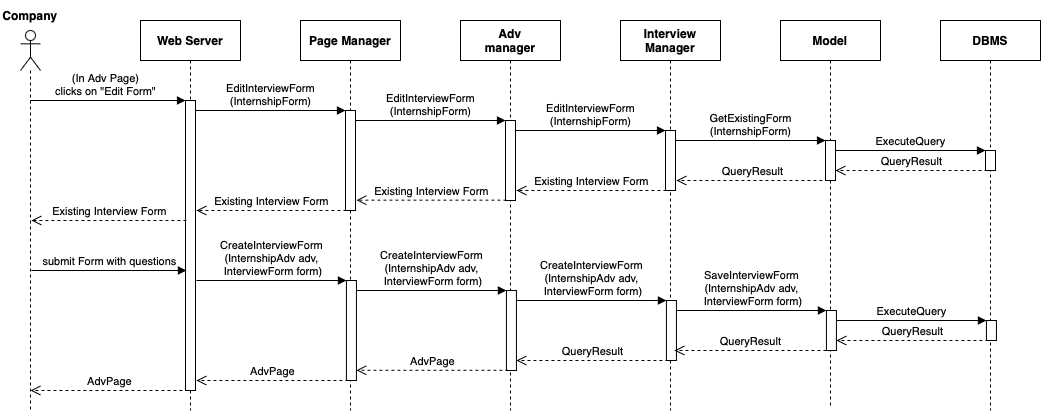
\includegraphics[width=15cm]{images/architectural design/runtime/DD-UC22.2.drawio.png}
    \caption{SD: Modify form for interview}
\end{figure}

\begin{figure}[H]
\textbf{Fill the form during interview}\newline\newline
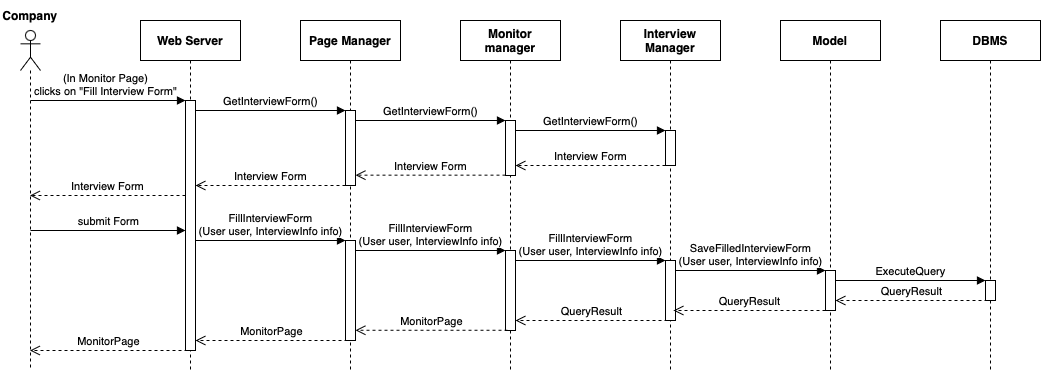
\includegraphics[width=15cm]{images/architectural design/runtime/DD-UC_23.drawio.png}
    \caption{SD: Fill the form during interview}
\end{figure}

\begin{figure}[H]
\textbf{Feedback}\newline\newline
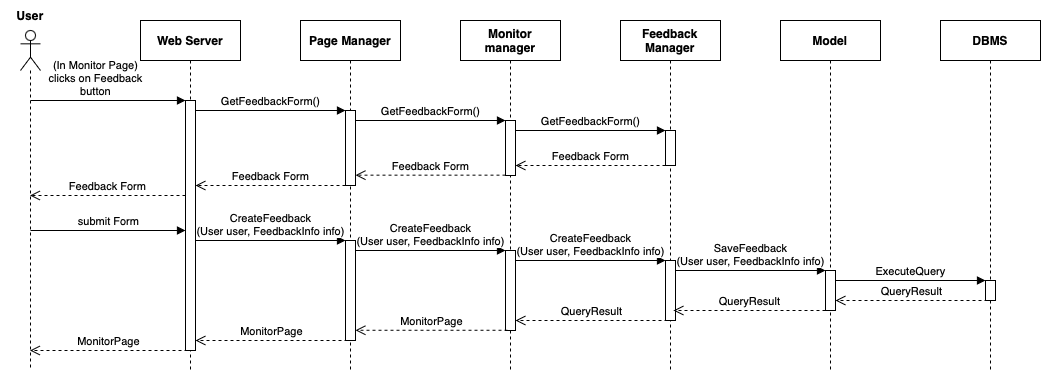
\includegraphics[width=15cm]{images/architectural design/runtime/DD-UC24_25.drawio.png}
    \caption{SD: Feedback}
\end{figure}

\begin{figure}[H]
\textbf{Monitoring}\newline\newline
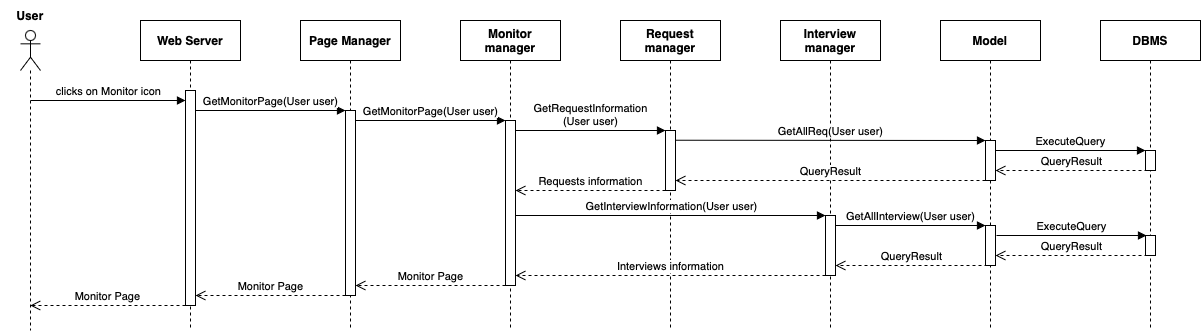
\includegraphics[width=15cm]{images/architectural design/runtime/DD-UC26_27_28.drawio.png}
    \caption{SD: Monitoring}
\end{figure}
\section{Component interfaces}

\begin{itemize}
    \item \textbf{Page Manager}
        \begin{itemize}
            \item It contains all the interfaces of all the others pages
        \end{itemize}
        
    \item \textbf{Registration Manager}
        \begin{itemize}
            \item GetStudentSingupPage()
            \item StudentSingup(String email, String university)
            \item StudentLogin(String email)
            \item GetCompanySingupPage()
            \item CompanySignup(String name, String VAT, File certificate, String email, File authorization)
            \item GetSetPasswordPage()
            \item InsertPassword(String password)
        \end{itemize}
        
    \item \textbf{Login Manager}
        \begin{itemize}
            \item GetStudentLoginPage()
            \item StudentLogin(String email)
            \item GetCompanyLoginPage()
            \item CompanyLogin(String username, String password)
        \end{itemize}
        
    \item \textbf{Request Manager}
        \begin{itemize}
            \item GetS2CRequestPage(Student student, Adv adv)
            \item FillS2CRequest(Student student, Adv adv, String message)
            \item GetC2SRequestPage(Company company, Student student)
            \item FillC2SRequest(Company company, Student student, Adv adv, String message)
            \item GetRequestInformation(User user)
            \item AcceptRequest(InternshipRequest req)
            \item RejectRequest(InternshipRequest req)
        \end{itemize}
        
    \item \textbf{Profile Manager}
        \begin{itemize}
            \item GetProfilePage(User user)
            \item UpdateCV(User user, File pdf)
            \item CheckPdfDimention(File pdf)
            \item AddCompetence(Map<CompetenceEnum, String> competences)
            \item EditCompetence(Competence competence, EnumCompetence type, String description)
        \end{itemize}
        
    \item \textbf{Interview Manager}
        \begin{itemize}
            \item GetInterviewInformation(User user)
            \item GetInterviewForm()
            \item FillInterviewForm(User user, InterviewInfo info)
            \item EditInterviewForm(InternshipForm)
            \item BlankInterviewForm()
            \item CreateInterviewForm(InternshipAdv adv, InterviewForm form)
            \item DeleteForm(InternshipAdv adv)
            \item NewInterviewPropose(InternshipAdv adv, Student student)
            \item GetProposeForm()
            \item GetInterviewPropose(InternshipAdv adv, Student student)
            \item AcceptProposal(InternshipAdv adv, Student student)
            \item RejectProposal(InternshipAdv adv, Student student)
        \end{itemize}
        
    \item \textbf{Adv Manager}
        \begin{itemize}
            \item GetADVsPage(Company company)
            \item GetNewADVForm()
            \item CreateADV(Company company, String name, String location, String profile, String project, String terms)
            \item CheckADV(Adv adv)
            \item GetADVPage(Adv adv)
            \item CreateADV(Company company, String name, String location, String profile, String project, String terms)
            \item EditCompetence(Competence competence, EnumCompetence type, String description)
            \item DeleteADV(Adv adv)
        \end{itemize}
        
    \item \textbf{Inbox Manager}
        \begin{itemize}
            \item GetInboxPage()
        \end{itemize}
        
    \item \textbf{Search Manager}
        \begin{itemize}
            \item GetSearchPage(User user)
            \item InsertInternshipFeatures(User user, List<String> features)
            \item InsertCandidateFeatures(User user, List<String> features)
            \item ElaborateSearchResults(List<Adv> results, List<Match> matches)
        \end{itemize}
        
    \item \textbf{Recommendation Manager}
        \begin{itemize}
            \item GetRecommendationPage(Recommendation recommendation) 
        \end{itemize}
        
    \item \textbf{Match Manager}
        \begin{itemize}
            \item CreateMatch(Internship req)
        \end{itemize}
        
    \item \textbf{Monitor Manager}
        \begin{itemize}
            \item GetMonitorPage(User user)
        \end{itemize}
        
    \item \textbf{Feedback Manager}
        \begin{itemize}
            \item GetFeedbackForm()
            \item CreateFeedback(User user, FeedbackInfo info)
        \end{itemize}
        
    \item \textbf{Model}
         \begin{itemize}
            \item CheckStudent(String email)
            \item CheckUniversity(String university)
            \item CheckCompany(String VAT)
            \item UpdateCompanyInfo(String username, String password)
            \item CheckCompany(String username, String password)
            \item GetUserInfo(User user)
            \item UpdateCV(User user, File pdf)
            \item AddCompetence(Map<CompetenceEnum, String> competences)
            \item EditCompetence(Competence competence, CompetenceEnum type, String description)
            \item GetADVsInfo(Company company)
            \item CreateADV(Company company, String name, String location, String profile, String project, String terms)
            \item GetADVInfo(Adv adv)
            \item EditCompetence(Competence competence, EnumCompetence type, String description)
            \item DeleteADV(Adv adv)
            \item GetUserSuggestedSearch(User user)
            \item GetSearchResult(List<String> features)
            \item GetStudentMatches(Student student)
            \item GetCompanyInfo(Adv adv)
            \item SaveS2CRequest(Student student, Adv adv, String message)
            \item SaveC2SRequest(Company company, Student student, Adv adv, String message)
            \item GetCompanyMatches(Company company)
            \item SaveSearchFields(Student student, List<String> fields)
            \item GetAllInterview(User user)
            \item GetAllReq(User user)
            \item SaveFeedback(User user, FeedbackInfo info)
            \item SaveInterviewForm(InternshipAdv adv, InterviewForm form)
            \item GetExistingForm(InternshipForm)
            \item SaveFilledInterviewForm(User user, InterviewInfo info)
            \item DeleteInterviewForm(InternshipAdv adv)
            \item GetInbox
            \item SaveInterviewPropose(InternshipAdv adv, Student student)
            \item DeleteInterviewProposal(InternshipAdv adv, Student student)
            \item NewMatch(Internship req)
            \item RequestRejected(InternshipRequest req)
        \end{itemize}   
\end{itemize}

\section{Selected architectural styles and patterns}
\label{subsec: 2.6 Selected architectural styles and patterns}
The S\&C system uses a combination of architectural styles and design patterns to ensure modularity, scalability, and maintainability. The core of the system is built around \textbf{Micro-service Architecture} and is integrated with a \textbf{3-Tier Architecture} and a \textbf{Client-Server Model}. These enable the system to meet performance and goals while maintaining flexibility.
\subsection{Micro-service Architecture}
The Micro-service Architecture divides the application into independent service, each one responsible for a specific functionality. It enables efficient development, testing, deployment, and scaling thanks to its modularity, each micro-service operates independently, communicating with other through APIs. A unified \textbf{API Gateway} serves as a centralised entry point for client requests, reducing direct interactions between clients and individual micro-services.
\subsection{3-Tier Architecture}
The 3-Tier Architecture is a software design model that organises the application into three layers. This model ensures modularity (each tier can be developed individually), scalability, maintainability (the separation of concerns allows for easier debugging), and security (it isolates the data, so the direct access to it is restricted). The three layers are:
\begin{enumerate}
    \item \textbf{Presentation Tier}, i.e. the user interface layer: this tier displays information to users and collects their input. In the S\&C platform, it is represented by the web pages and is located on the Web Server node of the physical architecture. This layer interacts with the micro-service through the unified API Gateway.
    \item \textbf{Application Tier}, i.e. the business logic layer: This tier contains the function to process input, execute decisions, and perform computations. It works as a bridge between the first and third layers. In the S\&C system is represented through the Model and is placed on the Application Server node. It ensures efficient data processing and coordination among micro-services.
    \item \textbf{Data Tier}: this tier stores and manages data through databases.
\end{enumerate}
\subsection{Client-Server Model}
The communication framework is developed following the Client-Server Model. The client is the web browser, it sends requests to the server using HTTPS protocol. The server processes the client's requests and provides responses. The Presentation Tier formats the server's responses while the Application Tier processes the client's requests.

\section{Other design decisions}
\subsection{Scalability}
The micro-services architecture implementation, as opposite at the monolithic one, enable a fine-gained scaling strategies, allowing a flexible deployment and more over a selective replication. Accordingly, with this approach we are able to scale the individual components rather than the entire system.

\subsection{Ease of Deployment}
The micro-services approach allows to enhance the ease of deployment, working with many smaller components, rather that a single big one, we can easily update them, test them and deploy them independently and, more over we can update and deploy the single components in parallel. Furthermore, with this approach we reduce the risks of critical errors, which can also be repaired easily in case they occur.